%%%%%%%%%%%%%%%%%%%%%%%%%%%%%%%%%%%%%%%%%%%%%%%%%%%%%%%%%%%%%%%%%%%%
%% I, the copyright holder of this work, release this work into the
%% public domain. This applies worldwide. In some countries this may
%% not be legally possible; if so: I grant anyone the right to use
%% this work for any purpose, without any conditions, unless such
%% conditions are required by law.
%%%%%%%%%%%%%%%%%%%%%%%%%%%%%%%%%%%%%%%%%%%%%%%%%%%%%%%%%%%%%%%%%%%%

\documentclass[
  digital,     %% Submit digital version. Change to `printed` for print.
  oneside,     %% One-sided for digital submission. Change to `twoside` for print.
  nosansbold,
  nocolorbold,
  lof,         %% Print List of Figures. Replace with `nolof` to hide.
  lot,         %% Print List of Tables.  Replace with `nolot` to hide.
]{fithesis4}

%% Locale (pdfLaTeX variant — matches Overleaf compiler setting)
\usepackage[resetfonts]{cmap}
\usepackage[T1]{fontenc}
\usepackage[
  main=english,
  english, czech, slovak
]{babel}

%% Thesis metadata
\thesissetup{
    date        = \the\year/\the\month/\the\day,
    university  = mu,
    faculty     = fi,
    type        = mgr,
    department  = Department of Software Engineering,
    author      = Bc. Jakub Sikula,
    gender      = m,
    advisor     = {RNDr. Tomáš Rebok, Ph.D.},
    title       = {Design and Implementation of a Platform for Real-Time Environmental Sensor Data Collection, Integration, and Visualisation},
    TeXtitle    = {Design and Implementation of a Platform for Real-Time Environmental Sensor Data Collection, Integration, and Visualisation},
    keywords    = {sensor data, environmental monitoring, IoT, MQTT, OGC SensorThings API, FastAPI, Next.js, TimescaleDB, Keycloak},
    TeXkeywords = {sensor data, environmental monitoring, IoT, MQTT, OGC SensorThings API, FastAPI, Next.js, TimescaleDB, Keycloak},
    abstract    = {%
      % TODO: Write the abstract (150--250 words).
      This thesis designs and implements a platform for real-time environmental sensor data collection,
      integration, and visualisation, targeting the operational needs of Czech University of Life Sciences
      Prague (CZU) within the context of the European eLTER long-term ecosystem research infrastructure.
      The work builds on the UFZ Time.IO solution as a foundation, addresses its identified limitations,
      and contributes the \texttt{water-dp} application layer and the \texttt{hydro-deploy} unified
      deployment orchestrator. TODO: complete this abstract.
    },
    thanks      = {%
      % TODO: Write acknowledgements.
      I would like to thank my advisor, RNDr. Tom\'{a}\v{s} Rebok, Ph.D., for his guidance throughout this work.
      TODO: complete acknowledgements.
    },
    bib         = thesis.bib,
    facultyLogo = fithesis-fi,
}

%% Packages
\usepackage{makeidx}
\makeindex
\usepackage{paralist}     %% Compact list environments
\usepackage{amsmath}      %% Mathematics
\usepackage{amsfonts}
\usepackage{url}          %% URLs in bibliography
\usepackage{listings}     %% Source code listings
\usepackage{booktabs}     %% \toprule, \midrule, \bottomrule in tables
\usepackage{tabularx}     %% Auto-width table columns
\usepackage{longtable}    %% Tables that span multiple pages
\usepackage{floatrow}     %% Captions above tables
\usepackage[babel]{csquotes} %% Context-sensitive quotation marks
\usepackage{tikz}         %% Diagrams and figures
\usetikzlibrary{shapes, arrows.meta, positioning, fit, backgrounds, calc}
%% microtype is already loaded by fithesis4 with [final,babel,nopatch=item]
\usepackage{pdflscape}     %% Landscape pages in portrait document

\floatsetup[table]{capposition=top}

%% Allow line breaks inside \texttt (monospace) text
\newcommand{\origtt}{}
\let\origtt\texttt
\renewcommand{\texttt}[1]{\origtt{\hyphenchar\font=`\-\relax #1}}
%% Slightly relax line-breaking tolerance to avoid overfull hboxes
\tolerance=1500
\emergencystretch=1.5em

\lstset{
  basicstyle      = \ttfamily\small,
  identifierstyle = \color{black},
  keywordstyle    = \color{blue},
  stringstyle     = \color{teal},
  commentstyle    = \itshape\color{magenta},
  breaklines      = true,
  frame           = single,
  numbers         = left,
  numberstyle     = \tiny\color{gray},
}

\begin{document}

\chapter*{Introduction}
\markright{\textsc{Introduction}}
\addcontentsline{toc}{chapter}{Introduction}
\label{chap:intro}

Environmental sensor networks have become essential infrastructure for understanding natural and built environments.
They operate across a wide range of domains: river gauging stations and catchment areas track water level, discharge,
and quality; urban installations measure air pollution, noise, and microclimate in cities; agricultural plots record
soil moisture, nutrient levels, and crop growth; biodiversity surveys deploy acoustic and camera-trap sensors in
forests and wetlands; and unmanned aerial vehicles carry multispectral or LiDAR payloads over landscapes that are
difficult to instrument permanently. Each of these domains produces continuous streams of heterogeneous data from
devices manufactured by different vendors, communicating over different protocols, and structured according to
different data models.

Managing this diversity at scale, from data acquisition in the field through ingestion, quality control, storage,
and visualization, is a non-trivial engineering problem. Environmental research institutions, national park
authorities, water management agencies, and university departments all face the same challenge: integrating
sensors across geographically distributed sites into a single, standards-compliant data infrastructure.

Czech University of Life Sciences Prague (CZU) is one such institution. As a university focused on life sciences,
agriculture, and environmental research, CZU operates sensor infrastructure spanning river gauging stations,
catchment monitoring networks, and experimental field plots, with instruments recording water level, conductivity,
temperature, turbidity, and other environmental parameters. Prior to this work, no unified platform existed to manage
this infrastructure in a coherent, standards-compliant way.

The UFZ Time.IO solution, developed at the Helmholtz Centre for Environmental Research in Leipzig, was identified as a
candidate foundation. Rather than building a full environmental data management system from scratch, this thesis
investigates whether Time.IO can be adapted to meet the operational requirements of a real institutional deployment,
and implements the extensions needed to close the gap between the upstream system and those requirements.

The platform must also be positioned within the broader context of the eLTER research
infrastructure, for which Time.IO serves as the time-series data acquisition component.
The CZU deployment therefore serves a dual purpose: it addresses a concrete operational
need at CZU, and it provides evidence for or against the suitability of the adapted
platform for wider eLTER adoption.

\medskip\noindent
The goals of this thesis are:
\begin{enumerate}
  \item To analyze the capabilities and limitations of the UFZ Time.IO system with respect to the CZU and eLTER
        deployment requirements.
  \item To design and implement the Water Data Platform (repository \texttt{water-dp}),
        an application layer providing project-oriented sensor management,
        MQTT-driven alert evaluation, geospatial integration, and a multilingual user portal.
  \item To implement a unified deployment layer (repository \texttt{hydro-deploy})
        enabling single-command installation of the complete integrated stack.
  \item To evaluate the resulting platform against the identified requirements and reflect on its suitability for
        broader adoption within the eLTER infrastructure.
\end{enumerate}

\medskip\noindent
The thesis follows a progression from understanding the problem domain to building and validating a solution.
Chapter~\ref{chap:background} first establishes the necessary context: the landscape of environmental sensor data
management, the OGC SensorThings API standard on which the platform relies, the upstream UFZ Time.IO system that
serves as the foundation, the institutional context linking the CZU deployment to the eLTER network through the
Time.IO adoption, and the eLTER research infrastructure whose data integration requirements constrain the design. This background
is essential because the design decisions in later chapters depend directly on the capabilities and constraints of
these existing technologies.

Building on this foundation, Chapter~\ref{chap:requirements} translates the CZU operational needs into concrete
requirements and performs a gap analysis against the baseline Time.IO system. The gaps identified here determine
the scope of the implementation work that follows.

Chapter~\ref{chap:architecture} then presents the architecture designed to close those gaps, explaining how
the two runtime layers, the inherited TSM ingestion infrastructure and the new
data platform application layer, interact and why they are structured as separate but integrated components.
Chapter~\ref{chap:implementation} justifies the major technology selections and describes the
realization of this architecture, including the unified deployment layer.

Finally, Chapter~\ref{chap:testing} evaluates the resulting platform against the requirements defined earlier,
verifying that the identified gaps have been addressed and assessing the platform's readiness for production
deployment.
Chapter~\ref{chap:conclusion} summarizes the contributions, reflects on limitations, and outlines future work.

\chapter{Background and Related Work}
\label{chap:background}

Later chapters build on several technologies and prior systems described here.
Section~\ref{sec:bg-sensor-data} reviews environmental sensor data management and its key challenges.
The OGC SensorThings API standard along with its FROST-Server implementation are covered in
Section~\ref{sec:bg-sta}. Section~\ref{sec:bg-timeio} then analyzes the UFZ Time.IO solution
that served as the starting point for the work. The institutional context behind its selection
is discussed in Section~\ref{sec:bg-elter-context}, and Section~\ref{sec:bg-elter} outlines
the eLTER research infrastructure and its data integration requirements.

%% ================================================================
\section{Environmental Sensor Data Management}
\label{sec:bg-sensor-data}
%% ================================================================

Environmental monitoring deployments typically connect sensors to data loggers or gateways
that forward observations to a central infrastructure. A representative architecture has four layers:
edge devices sampling physical quantities, an ingestion layer receiving data over one or more
protocols, a storage layer optimized for time-series workloads, and an access layer exposing the
data through standardized interfaces \cite{hart2006environmental}.

Heterogeneity across these systems poses a significant engineering challenge. A single monitoring network
may combine sensors from different manufacturers, each using a proprietary payload format, delivered
over MQTT, HTTP~POST, SFTP file upload, or manual CSV import. Temporal resolutions range from
sub-second sampling on vibrating-wire piezometers to daily aggregates from weather stations.
Reconciling these differences into a unified data model is a prerequisite for any cross-site analysis
\cite{horsburgh2008observations}.

Several platforms address parts of this problem space. The Observations Data Model~2 (ODM2)
\cite{horsburgh2016odm2} provides a relational schema for managing diverse observational data with
rich provenance metadata. ERDDAP \cite{simons2023erddap} focuses on data distribution, enabling
scientists to access gridded and tabular datasets through uniform query interfaces. The OGC Sensor
Observation Service (SOS) \cite{ogcsos} defines a standard web-service interface for querying sensor
data, but its XML-based protocol has been largely superseded by the RESTful SensorThings~API discussed
in Section~\ref{sec:bg-sta}.

What these solutions share is the recognition that interoperability standards are essential for
cross-institutional data sharing. Without a shared data model and access protocol, each
integration turns into a bespoke point-to-point effort. The work in this thesis focuses on
the Czech University of Life Sciences Prague (CZU) deployment, where sensors from multiple
manufacturers need to be unified under a single platform accessible to several research groups.

%% ================================================================
\section{OGC SensorThings API}
\label{sec:bg-sta}
%% ================================================================

The OGC SensorThings API (STA) \cite{ogc-sta} is an open standard that defines a RESTful interface
for managing and accessing Internet of Things sensor data. Ratified by the Open Geospatial Consortium in 2016,
it was designed to be lightweight, JSON-based, and suitable for resource-constrained IoT environments ---
in contrast to the earlier XML-heavy Sensor Observation Service.

\subsection{Data Model}
\label{sec:bg-sta-model}

The STA data model is built around six core entity types and their relationships:

\begin{itemize}
  \item \textbf{Thing} --- a physical object of interest, such as a weather station or a water gauge.
        A Thing has a \emph{Location} representing its geospatial position.
  \item \textbf{Datastream} --- a logical grouping of Observations measuring a single
        \emph{ObservedProperty} (e.g.\ water level, air temperature) with a specific \emph{Sensor}.
        Each Datastream belongs to exactly one Thing.
  \item \textbf{Observation} --- an individual measurement event, characterized by a
        \texttt{phenomenonTime} (when the phenomenon occurred), a \texttt{resultTime} (when the
        result was produced), and a \texttt{result} value.
  \item \textbf{Sensor} --- the instrument or procedure that produces Observations.
  \item \textbf{ObservedProperty} --- the physical quantity being measured (e.g.\
        ``Water Temperature'').
  \item \textbf{FeatureOfInterest} --- the real-world feature to which an Observation applies,
        typically derived from the Thing's Location.
\end{itemize}

The standard supports navigation between entities through URL-based association links. For example,
\texttt{/Things(1)/Datastreams} returns all Datastreams belonging to Thing~1, and
\texttt{/Datastreams(5)/Observations?\$filter=phenomenonTime gt 2024-01-01T00:00:00Z}
returns filtered Observations. This query model enables clients to traverse the entity graph
without prior knowledge of the underlying database schema.

STA also defines an MQTT extension (Part~2 of the standard) that allows clients to subscribe to
entity changes in real time, making it suitable for both historical queries and live data streams.

\subsection{STA Server Implementations}
\label{sec:bg-frost}

Several server implementations of the OGC SensorThings API exist. GOST\footnote{GOST SensorThings API server: \url{https://github.com/gost/server}} is a lightweight Go-based implementation focusing on ease of deployment and low resource consumption, but it implements only a subset of the query options and has seen limited maintenance since 2020. SensorThingsServer by 52°North\footnote{52°North SensorThings API: \url{https://github.com/52North/sensorweb-server-sta}} provides STA Part~1 compliance on top of Spring Boot and Hibernate, targeting integration with the broader 52°North sensor web ecosystem, though its community adoption remains smaller. FROST-Server \cite{frost-server}, developed by the Fraunhofer Institute for Optronics, System Technologies and Image Exploitation (IOSB), is the most widely adopted STA implementation and serves as the OGC reference for conformance testing.

FROST-Server was selected for this platform for three reasons. First, the upstream Time.IO system (Section~\ref{sec:bg-timeio}) already integrates FROST-Server, so adopting a different implementation would have required replacing a core component of the inherited stack. Second, FROST-Server provides full STA Part~1 (Sensing) compliance, including \texttt{\$filter}, \texttt{\$expand}, \texttt{\$select}, \texttt{\$orderby}, and \texttt{\$top}/\texttt{\$skip} query options, as well as the MultiDatastream extension for sensors producing multiple observed properties in a single observation. Third, a key architectural property of FROST-Server is that it reads entity data from PostgreSQL views rather than requiring a specific physical table layout. This allows operators to map an existing database schema to the STA entity model by defining appropriate SQL views, a capability that the Time.IO platform exploits through its local STA views, as described in Section~\ref{sec:bg-timeio-arch}.

FROST-Server is deployed as a Java web application on Apache Tomcat\footnote{Apache Tomcat: \url{https://tomcat.apache.org/}} and uses PostgreSQL\footnote{PostgreSQL: \url{https://www.postgresql.org/}} with the PostGIS\footnote{PostGIS spatial extension: \url{https://postgis.net/}} extension as its backing store. Each deployment is configured through a Tomcat context file that specifies the JDBC connection parameters, API version, and plugin settings.

%% ================================================================
\section{The UFZ Time.IO Solution}
\label{sec:bg-timeio}
%% ================================================================

Time.IO (internally referred to as \emph{tsm-orchestration} or TSM) is an open-source environmental
sensor data management platform developed at the Helmholtz Centre for Environmental Research (UFZ)
in Leipzig \cite{bumberger2025timeio,timeio-ref}. It provides an end-to-end pipeline for ingesting, storing,
quality-controlling, and serving environmental time-series data. The platform served as the starting
point for the work described in this thesis.

\subsection{The UFZ TSM Ecosystem}
\label{sec:bg-timeio-ecosystem}

Not a single repository, the UFZ TSM project is a broader ecosystem of over a dozen
components hosted under the \texttt{ufz-tsm} group on the Helmholtz Codebase. The ecosystem comprises three core components, illustrated in Figure~\ref{fig:timeio-ecosystem}: the Sensor Management System (SMS) for metadata registration and management, Time.IO for time-series data ingestion and storage, and the System for automated Quality Control (SaQC) for data analysis and quality assurance. Data enters the system via MQTT or (S-)FTP and is served through the OGC SensorThings API.

\begin{figure}[ht]
  \centering
  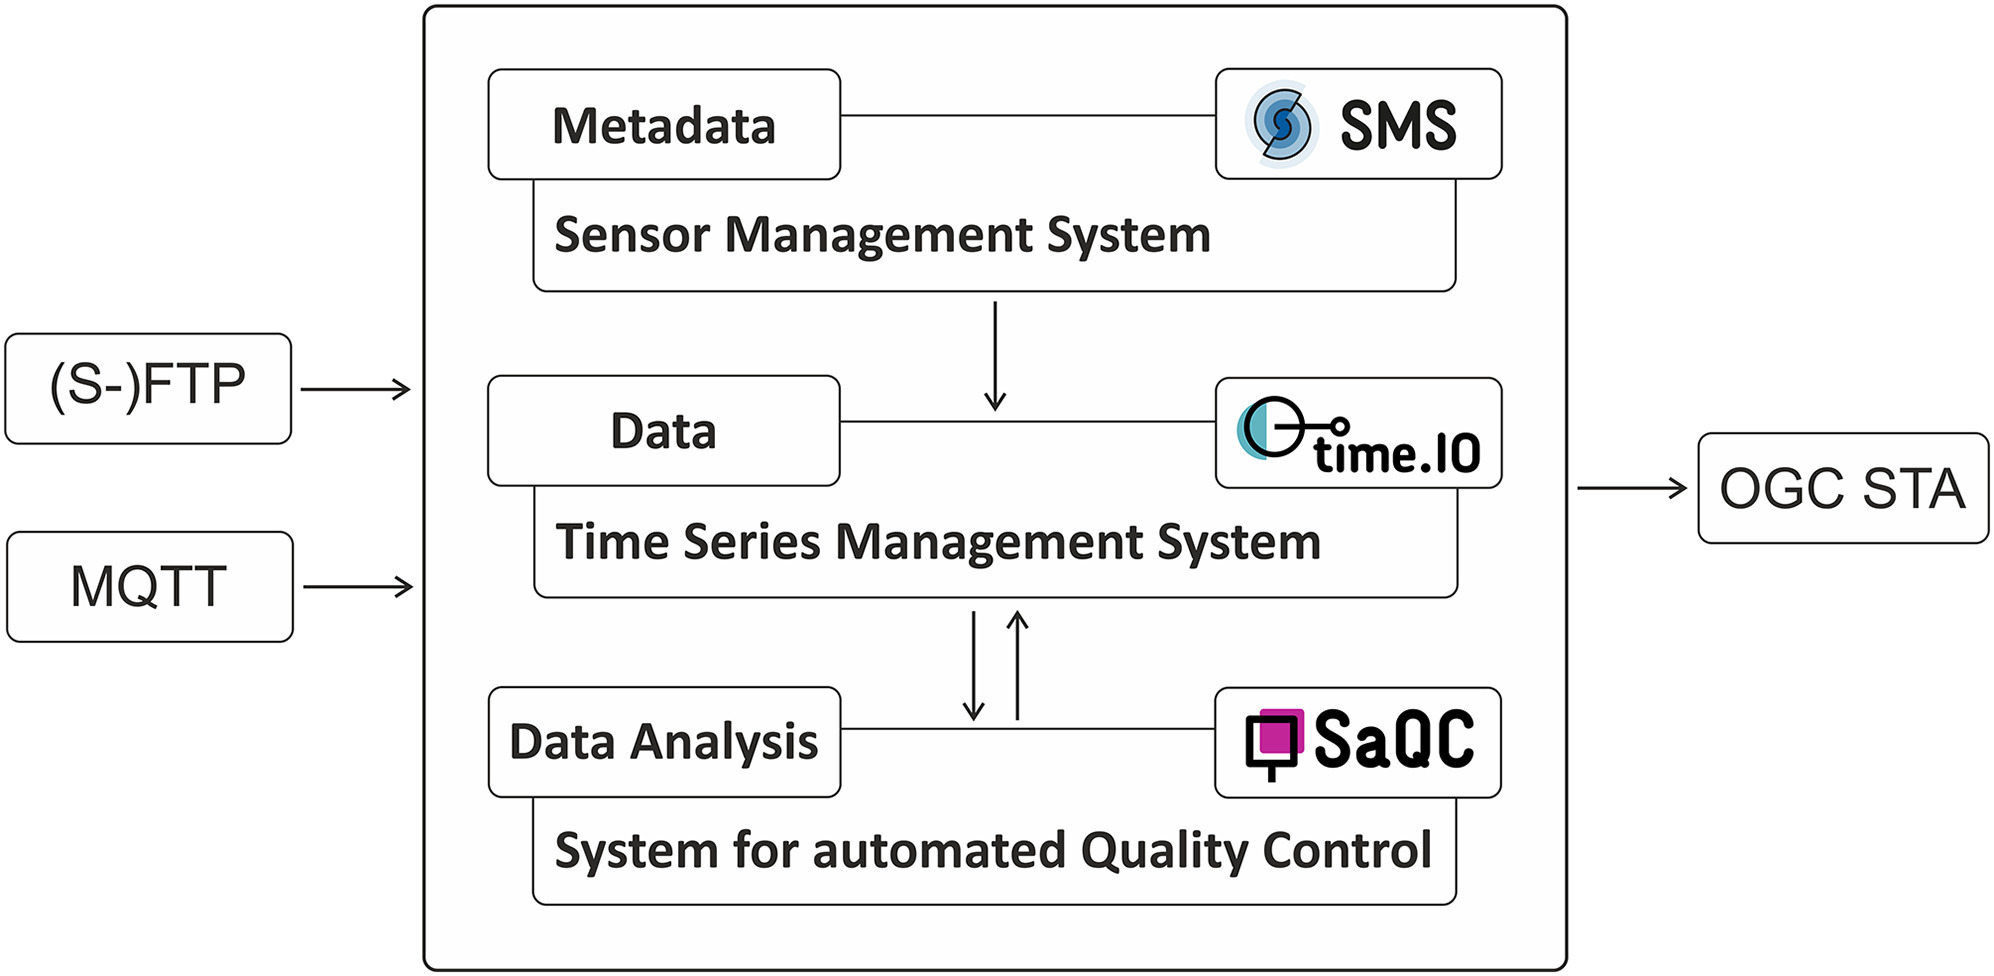
\includegraphics[width=0.85\textwidth]{figures/timeio-ecosystem.jpg}
  \caption{High-level architecture of the UFZ Time.IO ecosystem. \emph{Source: Bumberger et~al.\ \cite{bumberger2025timeio}, reproduced under CC-BY~4.0.}}
  \label{fig:timeio-ecosystem}
\end{figure}

Beyond the
core \texttt{tsm-orchestration} ingestion pipeline adopted in this thesis, the ecosystem
includes two frontend projects (\texttt{tsm-frontend}, a Django\footnote{Django web framework: \url{https://www.djangoproject.com/}} application with 465~commits,
and \texttt{thing-management}, a newer FastAPI/Vue.js\footnote{Vue.js framework: \url{https://vuejs.org/}} replacement started in September~2024),
a combined deployment repository (\texttt{timeio-and-sms}), the external Sensor Management
System (SMS) discussed in Section~\ref{sec:bg-timeio-limitations}, Kubernetes Helm charts,
developer utilities, and several supporting libraries.

This thesis adopts only \texttt{tsm-orchestration} as its foundation. The upstream frontend
components were replaced by the Water Data Platform portal (Chapter~\ref{chap:implementation})
because both upstream frontends produced invalid MQTT configuration messages that broke the
ingestion pipeline, and neither provided the project-oriented management model required by CZU.

\subsection{Architecture Overview}
\label{sec:bg-timeio-arch}

Time.IO is deployed as a set of Docker containers orchestrated by Docker Compose\footnote{Docker Compose: \url{https://docs.docker.com/compose/}}. The infrastructure
layer comprises the following core services:

\begin{itemize}
  \item \textbf{PostgreSQL with TimescaleDB} --- the central database, storing both the configuration
        database (\texttt{config\_db} schema) and per-thing observation data in isolated schemas.
  \item \textbf{Mosquitto\footnote{Eclipse Mosquitto MQTT broker: \url{https://mosquitto.org/}} MQTT broker} --- the event backbone connecting all workers and external
        sensor data sources. Supports both plain (port~1883) and TLS-encrypted (port~8883)
        connections.
  \item \textbf{MinIO object storage} --- an S3-compatible store used for file-based data ingestion.
        Each Thing receives its own bucket for raw data files.
  \item \textbf{FROST-Server} --- an OGC SensorThings API endpoint deployed on Apache Tomcat,
        providing standardized read access to observation data through SQL views over per-thing
        schemas.
  \item \textbf{Keycloak} --- an OpenID Connect identity provider managing user authentication
        and role-based access control.
  \item \textbf{Grafana}\footnote{Grafana visualization platform: \url{https://grafana.com/}} --- a visualization layer with pre-configured dashboards for time-series
        exploration.
  \item \textbf{Flyway}\footnote{Flyway database migration tool: \url{https://flywaydb.org/}} --- a database migration tool that applies versioned SQL scripts to
        initialise and evolve the database schema.
\end{itemize}

On top of these infrastructure services, Time.IO deploys a set of specialized workers and a
configuration API. The workers follow a message-driven architecture: each subscribes to one or more
MQTT topics, performs its designated processing, and optionally publishes results to downstream
topics. This design decouples the components and allows independent scaling and deployment
of each worker.

Its configuration database (\texttt{config\_db} schema) stores the metadata that drives the entire
pipeline. Key tables include \texttt{thing} (sensor device definitions), \texttt{project} (logical
groupings of Things), \texttt{database} (connection credentials per project), \texttt{s3\_store}
(MinIO bucket configuration), \texttt{file\_parser} and \texttt{file\_parser\_type} (parser
definitions), \texttt{mqtt} and \texttt{mqtt\_device\_type} (MQTT ingestion settings), and
\texttt{ext\_api} and \texttt{ext\_sftp} (external data source configurations).

Central to this design is the \emph{per-thing schema} pattern: when a new Thing is provisioned,
the platform creates a dedicated PostgreSQL schema containing its own observation and
datastream tables. The full provisioning sequence and its isolation properties are described
in Section~\ref{sec:arch-db-perthings}.

Upstream FROST-Server integration relies on a set of SQL views
(\texttt{sql/sta\_views/}) that map the STA entity model to tables managed by the external
Sensor Management System (SMS). These views query SMS-provided metadata (device catalogs,
contact records, deployment actions, and datastream links) to construct the
\texttt{THINGS}, \texttt{DATASTREAMS}, \texttt{OBSERVATIONS}, and related entities that
FROST-Server reads. Because the SMS service was never operational
(Section~\ref{sec:bg-timeio-limitations}), these views returned empty result sets or failed
entirely, rendering the STA endpoint non-functional. Without a working STA layer, FROST-Server
could not serve any observation data, effectively breaking one of the platform's core access
interfaces.

\subsection{Worker Architecture}
\label{sec:bg-timeio-workers}

All workers inherit from the \texttt{AbstractHandler} base class defined in the \texttt{timeio.mqtt}
module. This base class manages the MQTT connection lifecycle, health-check heartbeats, and
structured error handling. Each worker subscribes to one or more MQTT topics, performs its
designated processing in the \texttt{on\_message} callback, and optionally publishes results
to downstream topics. This message-driven design decouples the components and allows
independent scaling and deployment.

The platform deploys nine workers covering configuration processing, infrastructure
provisioning, data ingestion (file-based and MQTT-based), quality control, and
synchronization with external data sources. A cron scheduler triggers periodic execution
of the synchronization workers. The full worker catalog with MQTT topics and
responsibilities is presented in Table~\ref{tab:tsm-workers}
(Section~\ref{sec:impl-tsm-workers}).

\subsection{Parser Framework}
\label{sec:bg-timeio-parsers}

The data parsing subsystem uses a pluggable architecture based on an abstract base class
(\texttt{AbcParser}) with concrete implementations registered in a parser map. The framework
distinguishes between file parsers (used by the file-ingest worker for uploaded CSV and JSON
files) and MQTT parsers (used by the mqtt-ingest worker for real-time device payloads).

File parsers include a general-purpose CSV parser (\texttt{CsvParser}), a JSON parser
(\texttt{JsonParser}), and a Pandas-based parser (\texttt{PandasParser}) for complex
tabular transformations. MQTT device parsers are specialized for specific hardware:
\texttt{ChirpStackGenericParser} handles LoRaWAN payloads from the ChirpStack\footnote{ChirpStack LoRaWAN network server: \url{https://www.chirpstack.io/}} network server,
\texttt{CampbellCr6Parser} processes GeoJSON-formatted data from Campbell Scientific CR6 loggers,
\texttt{YdocMl417Parser} handles Ydoc ML-417 water quality sensors, and
\texttt{BrightskyDwdApiParser} parses German Weather Service API responses. A
\texttt{SineDummyParser} generates synthetic sine-wave data for testing.

Each parser produces a list of \texttt{Observation} objects with fields for timestamp, value, origin,
position (identifying the Datastream), and column header. Observations support four result types:
boolean, number, string, and JSON.

Critically, all parsers and device types in the upstream platform are hardcoded in the Python
source code. Adding support for a new sensor model or file format requires implementing a new
parser class, registering it in the parser map, rebuilding the Docker image, and redeploying
the affected worker. There is no mechanism for operators or end users to define new parsers,
MQTT device types, or file-parsing configurations at runtime through a management interface.
The database schema also lacks extensibility: the \texttt{mqtt\_device\_type} and
\texttt{ext\_api\_type} tables have no metadata columns, so any device-specific configuration
must be baked into the parser source code. This rigidity is a significant limitation for
deployments that must accommodate diverse and evolving sensor hardware.

\subsection{Current State and Limitations}
\label{sec:bg-timeio-limitations}

At the time this work commenced, Time.IO exhibited several limitations that directly
motivated the contributions of this thesis. These limitations span the SMS integration, the
upstream frontend solutions, and the overall project maturity.

\paragraph{Sensor Management System.}
The most significant limitation concerned the Sensor Management System (SMS), an external metadata
service intended to provide controlled vocabularies, semantic annotations, and a catalog of sensor
descriptions. The SMS was designed to be the authoritative source of Thing metadata for FROST-Server,
with dedicated SQL views (\texttt{sql/sta\_views/}) mapping SMS-managed entities to the STA data model.
However, the SMS service was never operational. The synchronization worker
(\texttt{sync\_sms\_manager.py}) existed in the codebase, but the upstream SMS backend it depended on
was not available. Without populated SMS tables, the STA views returned empty result sets or failed
to execute, rendering FROST-Server unable to serve any observation data. This was not a minor feature
gap: the STA endpoint is a core access interface of the platform, and its absence made the upstream
TSM deployment effectively non-functional for any client expecting standards-compliant data access.

The \texttt{timeio-and-sms} combined deployment repository, which was intended to demonstrate
the integrated SMS and Time.IO workflow, proved impossible to deploy successfully. Multiple
dependencies were outdated or no longer available, and the solution contained breaking bugs that
prevented the services from starting. The repository's documentation was partially written in
German and reflected an internal prototype rather than a production-ready integration. With only
175~commits total and activity ceasing in July~2024, the combined SMS deployment did not represent
a viable path forward.

\paragraph{Upstream frontends.}
The original \texttt{tsm-frontend} (Django) provided basic Thing management functionality but
contained bugs that caused inconsistencies between the frontend configuration forms and the
ingestion pipeline's expectations. When a Thing was created or modified through the Django
interface, the resulting MQTT configuration messages did not always match the format and content
that the downstream workers (\texttt{configdb-updater}, \texttt{thing-setup}) expected, leading
to silent failures in infrastructure provisioning.

The newer \texttt{thing-management} replacement (Vue.js~3 + FastAPI) was still in early development
at the time of this work, with limited functionality and similar integration issues. The
frontend's MQTT message generation contained bugs that caused several core ingestion workflows
, particularly file-based ingestion and external API synchronization, to fail. Neither
upstream frontend provided project-based multi-tenancy, role-based access control beyond basic
Helmholtz~AAI group membership, alerting, geospatial layer management, or internationalization
--- all of which were required for the CZU deployment.

\paragraph{Upstream project activity.}
Beyond the specific component issues, the upstream TSM ecosystem showed an overall pattern of
fragmented development. The codebase was distributed across more than a dozen repositories with
varying levels of maturity. The FETA module (\texttt{timeio/feta.py}), which provides an ORM-like
abstraction over the configuration database, was actively maintained and central to the worker
architecture. However, higher-level management features were either absent, buggy, or spread
across multiple partially overlapping projects (\texttt{tsm-frontend} vs.\ \texttt{thing-management}).

The platform lacks several capabilities required for the CZU deployment: project-based
multi-tenancy with role-based access, an alert and notification system, geospatial layer management,
a user-facing portal for sensor configuration and data exploration, and batch CSV import with
configurable parsing. These gaps are analyzed in Chapter~\ref{chap:requirements} and addressed
by the contributions described in Chapters~\ref{chap:architecture} and~\ref{chap:implementation}.

%% ================================================================
\section{Institutional Context: eLTER and the Adoption of Time.IO}
\label{sec:bg-elter-context}
%% ================================================================

The eLTER network relies on a shared digital layer called the eLTER CyberInfrastructure
(eLTER~CI), described in Section~\ref{sec:bg-elter-ci}. The UFZ is a core contributor to
this infrastructure: it develops and operates Time.IO as the time-series data acquisition
component of the eLTER~CI, handling ingestion, storage, quality control, and STA-based
access for environmental observations. The work is carried out under the EU Horizon~2020
eLTER~PLUS project (Grant Agreement No.~871128, 2020--2025), which funds the build-up of
the eLTER~CI and its validation through pilot deployments at real monitoring sites across
Europe.

The Czech University of Life Sciences Prague (CZU) operates hydrological and meteorological
monitoring networks across several catchment areas in the Czech Republic and aspires to
join the eLTER network as a recognized site. Its data management requirements ---
consolidating heterogeneous sensors under a single standards-compliant platform with
project-based multi-tenancy --- overlap closely with what Time.IO was built to provide.
Within the eLTER~PLUS project, CZU's deployment was established as a pilot: a test of
whether Time.IO can serve operational needs beyond UFZ's own sites and whether the
resulting extensions can feed back into the shared eLTER~CI.

This pilot arrangement defines the scope of the thesis. The work builds on a fork of
\texttt{tsm-orchestration} rather than a new platform, and the extensions described in
later chapters are designed with upstream contribution in mind. Building on Time.IO ties
the CZU deployment into the broader eLTER adoption path, but it also means inheriting
the limitations documented in Section~\ref{sec:bg-timeio-limitations}.

%% ================================================================
\section{eLTER Research Infrastructure}
\label{sec:bg-elter}
%% ================================================================

The European Long-Term Ecosystem, Critical Zone and Socio-Ecological Research Infrastructure
(eLTER~RI) \cite{elter-ref} coordinates environmental monitoring across more than 400~sites
in over 25~European countries. Sites range from alpine observatories and forest flux towers
to freshwater catchments and urban gradient transects. The network distinguishes two
categories: \emph{eLTER Sites}, which carry out long-term observations at the ecosystem
level, and \emph{eLTER Platforms}, which host intensive, high-resolution measurement campaigns
on shorter time scales. eLTER is currently transitioning from project-funded development
under eLTER~PLUS toward sustained operation as a European Research Infrastructure
Consortium (ERIC).

\subsection{eLTER CyberInfrastructure}
\label{sec:bg-elter-ci}

Connecting these distributed sites into a coherent research environment is the
role of the eLTER CyberInfrastructure (eLTER~CI), developed under the eLTER~PLUS
project. The eLTER~CI is designed as an integrated service environment --- not a
loose federation of tools --- where data, metadata, and user-facing applications
share a common identity layer, aligned metadata structures, and coordinated
workflows spanning dataset submission through quality control, curation, discovery,
and analytical use.

The CI supports two complementary data pathways. On the \emph{provider side},
site operators submit datasets (or have them harvested from external repositories),
complete metadata according to an eLTER-specific profile, pass automated quality
checks, and publish records through a curator-mediated review. On the
\emph{consumer side}, researchers discover datasets by site or observed property,
inspect them against controlled vocabularies, access the data through
standardized service endpoints, and perform analysis in managed compute
environments. The main components that implement these pathways are:

\begin{itemize}
  \item \textbf{eLTER~LogIn} --- a federated identity and access service built on
        Perun~AAI, supporting institutional login via eduGAIN, EGI~Check-in, ORCID,
        and Google. A single consolidated identity per user spans all CI services,
        with role-based access control distinguishing data providers, curators,
        researchers, and administrators.
  \item \textbf{Digital Asset Register (DAR)} --- the central dataset repository,
        built on InvenioRDM. It handles registration, metadata curation (using an
        eLTER-specific metadata model), automated quality checks orchestrated by
        Argo~Workflows, and publication with DOI minting through DataCite. A
        harvesting subsystem retrieves metadata from external repositories
        (B2SHARE, Zenodo, and others) so that externally stewarded datasets
        also appear in the eLTER catalog.
  \item \textbf{DEIMS-SDR} --- the Site and Dataset Registry at
        \texttt{deims.org}, serving as the authoritative source of site-level
        metadata: geographic boundaries, instrumentation, observed properties,
        and responsible organizations. Dataset records in the DAR link to
        DEIMS-SDR site identifiers.
  \item \textbf{Vocabulary services} --- controlled terminologies (EnvThes for
        observed properties, eLTER Standard Observations, eLTER Controlled Lists)
        published through SKOSMOS and Apache Jena. These enable consistent
        semantic annotation across sites and disciplines.
  \item \textbf{Online data services} --- Time.IO (TimescaleDB-based) for
        time-series access and Spatial.IO (GeoServer-based) for geospatial
        layers, both linked to DAR records through an Online Asset Register (OAR)
        so that dataset metadata and data access remain connected.
  \item \textbf{DataLabs} --- a JupyterHub-based analytical environment running
        on the CI compute cluster, offering pre-built images (Python, R/RStudio,
        TensorFlow with optional GPU access) for dataset preprocessing,
        transformation, and exploratory analysis.
\end{itemize}

The entire stack runs on Kubernetes and is operated through a GitOps workflow,
making deployments reproducible and auditable. This architecture is directly
relevant to the present work: the CZU deployment is intended to function as a
site-level data acquisition node within the eLTER~CI, with observations
ingested through Time.IO ultimately discoverable and accessible through the DAR
and the associated online services.

\subsection{Implications for Site-Level Deployments}
\label{sec:bg-elter-implications}

Several properties of the eLTER~CI directly constrain what a site-level platform must provide.
Data served to the network must be accessible through the OGC SensorThings API, which the
eLTER~CI has adopted as its candidate standard for real-time sensor data. Sites must
describe their sensors and observed properties using eLTER's controlled vocabularies so that
cross-site queries return semantically comparable results. Authentication must support federated
identity providers compatible with the eLTER~LogIn service. At the same time, individual sites
retain operational independence --- they choose their own sensor hardware, data collection
procedures, and local infrastructure --- so the platform must accommodate heterogeneous
configurations rather than mandating a specific vendor or format.

The gaps between the current CZU deployment and a production-ready eLTER integration ---
including vocabulary alignment, cross-site federation, and FAIR metadata compliance ---
are assessed in Section~\ref{sec:test-deployment-elter}.

\chapter{Requirements Analysis}
\label{chap:requirements}

The requirements for the platform are derived from the CZU deployment context. A gap analysis
against the baseline Time.IO system then motivates the scope of the contributions.
Section~\ref{sec:req-usecases} identifies the CZU use cases and stakeholder
needs. Sections~\ref{sec:req-functional} and~\ref{sec:req-nonfunctional} enumerate the functional and non-functional
requirements respectively. Section~\ref{sec:req-gap} compares those requirements against the capabilities of the
original UFZ Time.IO system.

%% ================================================================
\section{CZU Use Cases and Stakeholder Needs}
\label{sec:req-usecases}
%% ================================================================

Czech University of Life Sciences Prague (CZU) operates environmental monitoring infrastructure
across river catchment monitoring projects and experimental plots. The primary stakeholders are
research groups responsible for individual monitoring projects, each of which manages a distinct
set of sensors and requires isolated data views with controlled access. Three actor roles interact
with the platform: \emph{Researcher} (creates projects, configures sensors, analyzes data),
\emph{Administrator} (manages users, groups, and platform-wide settings), and
\emph{External System} (automated data sources such as MQTT devices, SFTP servers, and external
APIs). An additional implicit actor is the \emph{TSM Ingestion Pipeline}, which provisions
infrastructure and processes data on behalf of the other actors.

The use cases are organized into three groups: data ingestion, platform management, and data
consumption. These groups are illustrated in Figures~\ref{fig:uc-ingestion},
\ref{fig:uc-management}, and~\ref{fig:uc-consumption}.

%% PlantUML source files live in figures/*.puml
%% Regenerate PDFs: plantuml -tpdf figures/*.puml

%% --- Use Case Diagram: Data Ingestion ---
\begin{figure}[htbp]
  \centering
  \includegraphics[width=0.85\textwidth]{figures/uc-ingestion.pdf}
  \caption{Use case diagram: data ingestion.}
  \label{fig:uc-ingestion}
\end{figure}

%% --- Use Case Diagram: Platform Management ---
\begin{figure}[htbp]
  \centering
  \includegraphics[width=0.85\textwidth]{figures/uc-management.pdf}
  \caption{Use case diagram: platform management.}
  \label{fig:uc-management}
\end{figure}

%% --- Use Case Diagram: Data Consumption ---
%% NOTE: UC-16 (Run computation) removed — feature decommissioned.
\begin{figure}[htbp]
  \centering
  \includegraphics[width=0.85\textwidth]{figures/uc-consumption.pdf}
  \caption{Use case diagram: data consumption.}
  \label{fig:uc-consumption}
\end{figure}

The identified use cases are summarized in Table~\ref{tab:usecases}.
%% UC-16 (Run computation) removed — feature decommissioned.

\begin{longtable}{l p{0.58\textwidth} p{0.18\textwidth}}
  \caption{Summary of use cases derived from the CZU deployment context.}
  \label{tab:usecases} \\
  \toprule
  ID & Description & Primary actor \\
  \midrule
  \endfirsthead
  \toprule
  ID & Description & Primary actor \\
  \midrule
  \endhead
  \midrule
  \multicolumn{3}{r}{\emph{Continued on next page}} \\
  \endfoot
  \bottomrule
  \endlastfoot
  UC-1  & Upload a CSV data file to a Thing's storage bucket for batch ingestion.
          The file is parsed using the Thing's configured parser and the resulting
          Observations are inserted into the per-thing schema. & Researcher \\
  UC-2  & Stream real-time MQTT data from a field sensor. The device publishes
          payloads to a topic namespace; the mqtt-ingest worker parses
          and stores the Observations. & MQTT Device \\
  UC-3  & Periodically synchronise files from an external SFTP server into a
          Thing's MinIO bucket, triggering file-ingest processing. & SFTP Server \\
  UC-4  & Periodically pull data from an external REST API (e.g.\ DWD, TTN)
          using a built-in or custom syncer script. & External API \\
  UC-5  & Onboard multiple sensors at once by uploading a CSV template containing
          Thing definitions, with per-row validation and error reporting. & Researcher \\
  UC-6  & Create, update, and delete projects. Assign members with roles
          (owner, editor, viewer) and link sensors to projects. & Researcher \\
  UC-7  & Configure a sensor: select ingest type, assign a parser,
          set MQTT credentials, define Datastream metadata, and specify
          geographic coordinates. & Researcher \\
  UC-8  & Define alert rules on a Datastream (threshold, no-data, computation
          failure) with severity levels (info, warning, critical).
          Acknowledge and resolve triggered alerts. & Researcher \\
  UC-9  & Configure QA/QC test pipelines per project using SaQC functions with
          tunable parameters. Trigger evaluation on demand. & Researcher \\
  UC-10 & Create and manage Keycloak groups and assign users to role-based
          subgroups (viewers, editors, admins). & Administrator \\
  UC-11 & Create and publish geospatial layers (vector, raster, WMS) through
          GeoServer with configurable access control. & Administrator \\
  UC-12 & Visualize time-series data for one or more Datastreams with
          interactive charts, decimation controls, and adjustable Y-axis bounds.
          & Researcher \\
  UC-13 & View sensor locations on an interactive map with color-coded markers
          and overlay geospatial layers. & Researcher \\
  UC-14 & Export Observation data as CSV for offline analysis. & Researcher \\
  UC-15 & Query the OGC SensorThings API endpoint for machine-to-machine data
          access using standard \texttt{\$filter} and \texttt{\$expand} queries. & External Client \\
\end{longtable}

%% ================================================================
\section{Functional Requirements}
\label{sec:req-functional}
%% ================================================================

The functional requirements are derived from the use cases in Section~\ref{sec:req-usecases}
and are grouped into eight areas. Each requirement is assigned an identifier for traceability
in Chapter~\ref{chap:testing}.

\subsection{Data Ingestion}
\label{sec:req-functional-ingestion}

\begin{description}
  \item[FR-1] The system shall ingest real-time sensor data via MQTT, supporting device-specific
    parsers that can be registered and selected per Thing. \emph{(UC-2)}
  \item[FR-2] The system shall ingest historical data from CSV files uploaded to a Thing's
    object-storage bucket, parsed using the Thing's configured file parser. \emph{(UC-1)}
  \item[FR-3] The system shall periodically synchronise data from external SFTP servers,
    downloading new files into the Thing's bucket for subsequent file-ingest processing.
    \emph{(UC-3)}
  \item[FR-4] The system shall periodically pull data from external REST APIs using built-in
    syncers (DWD, TTN, Bosch) or user-provided custom syncer scripts. \emph{(UC-4)}
  \item[FR-5] The system shall support uploading custom MQTT parser scripts and custom API
    syncer scripts, validated before deployment. \emph{(UC-2, UC-4)}
\end{description}

\subsection{Sensor Management}
\label{sec:req-functional-sms}

\begin{description}
  \item[FR-6] The system shall support creating, updating, and deleting Things with configurable
    ingest type (MQTT, SFTP, external API), parser assignment, and geographic coordinates.
    \emph{(UC-7)}
  \item[FR-7] The system shall allow bulk import of Thing definitions from a CSV file, with
    per-row validation and error reporting. A downloadable CSV template shall be provided.
    \emph{(UC-5)}
  \item[FR-8] The system shall track sensor activity per Thing, detecting inactivity based on
    a configurable threshold (default: 24~hours) and raising alerts when no data is received.
    \emph{(UC-8)}
  \item[FR-9] The system shall manage MQTT device types and CSV parser definitions as reusable
    catalog entries that can be assigned to multiple Things. \emph{(UC-7)}
\end{description}

\subsection{Project Management}
\label{sec:req-functional-projects}

\begin{description}
  \item[FR-10] The system shall support creating, updating, and deleting projects. Each project
    shall group a set of Things with shared access control. \emph{(UC-6)}
  \item[FR-11] The system shall support assigning users to projects with one of three roles:
    owner (full control), editor (modify data and configuration), or viewer (read-only access).
    \emph{(UC-6)}
  \item[FR-12] The system shall create a dedicated TimeIO database schema per project for
    per-thing observation storage. \emph{(UC-6)}
\end{description}

\subsection{Data Quality}
\label{sec:req-functional-quality}

\begin{description}
  \item[FR-13] The system shall support configuring QA/QC test pipelines per project, using
    functions from the SaQC (Statistical Quality Control) library with tunable parameters.
    \emph{(UC-9)}
  \item[FR-14] The system shall execute QA/QC tests automatically when new data is parsed
    (triggered by the \texttt{data\_parsed} MQTT event) and store quality flags alongside
    Observations. \emph{(UC-9)}
  \item[FR-15] The system shall allow on-demand triggering of QA/QC evaluation through the
    API. \emph{(UC-9)}
\end{description}

\subsection{Visualization}
\label{sec:req-functional-viz}

\begin{description}
  \item[FR-16] The system shall provide interactive time-series charts with support for multiple
    Datastream overlays, decimation controls for large datasets, and adjustable Y-axis bounds.
    \emph{(UC-12)}
  \item[FR-17] The system shall display sensor locations on an interactive map with color-coded
    markers and popup details. WMS/WFS geospatial layers shall be overlayable. \emph{(UC-13)}
  %% FR-18 removed — custom dashboards decommissioned.
  \item[FR-19] The system shall allow exporting Observation data as CSV files for offline
    analysis. \emph{(UC-14)}
\end{description}

\subsection{Authentication and Access Control}
\label{sec:req-functional-auth}

\begin{description}
  \item[FR-20] The system shall authenticate users via OpenID Connect (OIDC) through a
    Keycloak identity provider. User registration, login, token refresh, and password change
    shall be supported. \emph{(UC-6, UC-10)}
  \item[FR-21] The system shall enforce a two-tier role-based access control model:
    Tier~1 at the group level (viewer, editor, admin roles stored in Keycloak subgroups) and
    Tier~2 at the project level (owner, editor, viewer roles stored in the application database).
    Realm-level administrators shall override all restrictions. \emph{(UC-10)}
  \item[FR-22] The system shall support creating and managing Keycloak groups with role-based
    subgroups. Group membership shall propagate as default permissions for projects within
    the group. \emph{(UC-10)}
\end{description}

\subsection{Batch Import}
\label{sec:req-functional-batch}

\begin{description}
  \item[FR-23] The system shall allow uploading historical time-series data as CSV files
    (up to 200~MB) with automatic Datastream mapping. \emph{(UC-1)}
  \item[FR-24] The system shall allow importing geospatial data in GeoJSON format (up to
    200~MB) with streamed processing. \emph{(UC-11)}
\end{description}

\subsection{Multilingual Interface}
\label{sec:req-functional-i18n}

\begin{description}
  \item[FR-25] The user interface shall be available in English, Czech, and Slovak, with
    locale detection based on browser settings and manual override. \emph{(all use cases)}
\end{description}

%% ================================================================
\section{Non-Functional Requirements}
\label{sec:req-nonfunctional}
%% ================================================================

The non-functional requirements govern the operational and quality properties of the platform.

\begin{description}
  \item[NFR-1] \textbf{Containerized deployment.} The entire platform shall be deployable as
    Docker Compose services. Rootless Podman shall be supported as an alternative container
    runtime.

  \item[NFR-2] \textbf{OGC SensorThings API compliance.} The platform shall expose observation
    data through a FROST-Server instance that is fully compliant with OGC STA Part~1 (Sensing),
    including \texttt{\$filter}, \texttt{\$expand}, and \texttt{\$orderby} query parameters.

  \item[NFR-3] \textbf{OIDC standards compliance.} Authentication shall follow the OpenID Connect
    standard with JWT token validation, JWKS key rotation, and standard token endpoints.

  \item[NFR-4] \textbf{Modular extensibility.} New ingestion worker types, parsers, and API
    syncers shall be addable without modifying the core platform. Custom parsers and syncers shall
    be uploadable as Python scripts at runtime.

  \item[NFR-5] \textbf{Security.} User-uploaded parser and syncer scripts shall be sandboxed
    through AST-based validation that blocks dangerous operations (\texttt{eval}, \texttt{exec},
    \texttt{open}, \texttt{getattr}/\texttt{setattr}). API rate limiting shall protect
    authentication endpoints. Credentials stored in the database shall be encrypted.

  \item[NFR-6] \textbf{Maintainability.} The codebase shall use database migrations (Alembic
    for \texttt{water-dp}, Flyway for TSM) to manage schema evolution. The API shall generate
    OpenAPI documentation automatically.

  \item[NFR-7] \textbf{eLTER interoperability alignment.} The architecture shall support
    future extension toward eLTER metadata standards and cross-site federation without
    requiring a fundamental redesign.

  \item[NFR-8] \textbf{Unified deployment.} The combined TSM and \texttt{water-dp} stacks shall
    be deployable through a single configuration file and Makefile, with automated secret
    generation and health checks.
\end{description}

%% ================================================================
\section{Gap Analysis: Time.IO vs.\ Target Platform}
\label{sec:req-gap}
%% ================================================================

Table~\ref{tab:gap-analysis} summarizes the gap between the Time.IO baseline capabilities and the
requirements identified in Sections~\ref{sec:req-functional} and~\ref{sec:req-nonfunctional}.
Each row identifies a capability that the upstream Time.IO system does not provide, the specific
requirements it blocks, and the component that addresses the gap in this thesis.

\begin{longtable}{l p{0.58\textwidth} p{0.19\textwidth}}
  \caption{Gap analysis: Time.IO baseline vs.\ target platform requirements.}
  \label{tab:gap-analysis} \\
  \toprule
  Gap & Description & Addressed by \\
  \midrule
  \endfirsthead
  \toprule
  Gap & Description & Addressed by \\
  \midrule
  \endhead
  \midrule
  \multicolumn{3}{r}{\emph{Continued on next page}} \\
  \endfoot
  \bottomrule
  \endlastfoot

  G-1 & \textbf{No project-oriented data model.} Time.IO organizes Things by
        configdb projects (Keycloak groups), but provides no application-level
        project entity with member roles or sensor assignment.
        \emph{(FR-10--12)} & \texttt{water-dp} \\[6pt]

  G-2 & \textbf{No user-facing web portal.} The upstream frontends
        (\texttt{tsm-frontend}, \texttt{thing-management}) provide only basic
        Thing CRUD through Django or Vue.js admin interfaces. No unified portal
        with time-series visualization, map display, or alerting exists.
        \emph{(FR-16--19)} & \texttt{water-dp} \\[6pt]

  G-3 & \textbf{No geospatial layer management.} Time.IO stores geographic
        coordinates in the configdb but provides no GIS integration, layer
        publishing, or spatial query capabilities.
        \emph{(FR-17, FR-24)} & \texttt{water-dp} \\[6pt]

  G-4 & \textbf{Non-functional local STA views.} The original local STA views
        contained issues that prevented FROST-Server from returning valid
        responses for certain entity types.
        \emph{(NFR-2)} & TSM adaptation \\[6pt]

  G-5 & \textbf{Non-functional SMS service.} The Sensor Management System
        backend was not operational; the \texttt{timeio-and-sms} combined
        deployment was impossible to start due to broken dependencies.
        \emph{(FR-6, FR-9)} & TSM adaptation \\[6pt]

  G-6 & \textbf{No alert evaluation subsystem.} Time.IO provides no mechanism
        for threshold monitoring, no-data detection, or notification of
        anomalous conditions.
        \emph{(FR-8, UC-8)} & \texttt{water-dp} \\[6pt]

  G-7 & \textbf{No unified deployment mechanism.} The TSM and application
        stacks are separate Docker Compose deployments with no shared
        configuration, secret management, or health-check tooling.
        \emph{(NFR-1, NFR-8)} & \texttt{hydro-deploy} \\[6pt]

  G-8 & \textbf{No Podman rootless support.} The upstream Compose files use
        Docker-specific features (environment list format, disabled service
        references) that are incompatible with rootless Podman.
        \emph{(NFR-1)} & \texttt{hydro-deploy} \\[6pt]

  G-9 & \textbf{No multilingual interface.} The upstream frontends are
        English-only with no internationalization framework. Czech and Slovak
        language support is required for CZU users.
        \emph{(FR-25)} & \texttt{water-dp} \\[6pt]

  %% G-10 removed — computation framework decommissioned.

  G-11 & \textbf{Upstream frontend bugs.} Both \texttt{tsm-frontend} (Django)
         and \texttt{thing-management} (Vue.js) generated MQTT configuration
         messages that did not match the ingestion pipeline's expectations,
         causing silent provisioning failures.
         \emph{(FR-6, FR-7)} & \texttt{water-dp} \\[6pt]

  G-12 & \textbf{Hardcoded parsers and device types.} All file parsers, MQTT
         device-type parsers, and API syncers are implemented as Python classes
         compiled into the Docker image. Adding support for a new sensor model
         or file format requires source-code changes and redeployment; there is
         no runtime mechanism for users to register custom parsers or device
         types through a management interface.
         \emph{(FR-5, FR-9, NFR-4)} & \texttt{water-dp} \\

\end{longtable}

The eleven gaps identified in Table~\ref{tab:gap-analysis} define the scope of the three
contributions described in Chapters~\ref{chap:architecture} and~\ref{chap:implementation}:
the \texttt{water-dp} application layer addresses gaps~G-1--G-3 and G-6--G-9, G-11, and G-12,
the TSM adaptations address gaps~G-4 and~G-5, and the \texttt{hydro-deploy} deployment
orchestrator addresses gaps~G-7 and~G-8. Each gap is revisited in the requirements evaluation
in Chapter~\ref{chap:testing}.

\chapter{Architecture Design}
\label{chap:architecture}

The gaps identified in Chapter~\ref{chap:requirements} shaped the platform architecture
presented here. The design builds on the upstream Time.IO system
(Section~\ref{sec:bg-timeio}) as the infrastructure layer and adds a new application
layer on top. The components fall into three categories by provenance:

\begin{description}
  \item[Inherited (upstream).] Components taken from the UFZ Time.IO platform and
    used without modification: PostgreSQL/TimescaleDB, Mosquitto, MinIO, FROST-Server,
    Keycloak, Grafana, and Flyway.
  \item[Inherited and modified.] Components forked from upstream and extended or fixed
    as part of this thesis: the ingestion workers, the per-thing schema provisioning
    logic, the FROST-Server SQL views (replaced), and the configuration database schema
    (new migrations).
  \item[New.] Components designed and implemented entirely in this thesis: the
    Water Data Platform application layer (FastAPI backend, Next.js frontend, Celery
    worker, GeoServer integration), the alert system, the batch import pipeline,
    and the project-oriented data model.
\end{description}

Section~\ref{sec:arch-overview} lays out the
overall system design and the rationale behind the two-layer split.
Section~\ref{sec:arch-components} defines each component's responsibility boundaries.
The database design, including the per-thing schema pattern and the local STA views,
follows in Section~\ref{sec:arch-database}. Section~\ref{sec:arch-mqtt} details the
MQTT-driven event architecture.

%% ----------------------------------------------------------------
\section{Overall System Architecture}
\label{sec:arch-overview}
%% ----------------------------------------------------------------

The platform is composed of two runtime layers, illustrated in
Figure~\ref{fig:arch-overview}.

\begin{landscape}
\begin{figure}[p]
  \centering
  \begin{tikzpicture}[
    box/.style={draw, thick, minimum width=3.2cm, minimum height=1cm, align=center, font=\small},
    newbox/.style={box, fill=blue!8},
    modbox/.style={box, fill=orange!12},
    layer/.style={draw, thick, rounded corners=3pt, inner sep=14pt},
    arr/.style={-{Stealth[length=5pt]}, thick},
    lbl/.style={font=\scriptsize, fill=white, inner sep=2pt},
    every node/.style={font=\small}
  ]

    %% ═══════════════════════════════════════════════
    %% LAYOUT: 3 rows, 2cm gap between packages
    %%   wdp:  x = -0.5 … 6.5   (center 3,   w=7cm)
    %%   tsm:  x =  8.5 … 15.5  (center 12,  w=7cm)
    %%   gap:  x =  6.5 … 8.5   (clear channel)
    %%   data: x =  0.5 … 14.5  (center 7.5, w=14cm)
    %% ═══════════════════════════════════════════════

    %% ── Researcher ──
    \node[font=\normalsize\bfseries] (user) at (7.5, 1) {Researcher};

    %% ── water-dp (label above-left, away from arrow landing) ──
    \node[layer, fill=blue!4] (wdp) at (3, -3.5) [minimum width=7cm, minimum height=5cm] {};
    \node[font=\small\bfseries, anchor=south west] at (wdp.north west) {Water Data Platform (application layer)};
    \node[newbox] (frontend) at (1.2, -2.2) {Next.js\\Frontend};
    \node[newbox] (api)      at (4.8, -2.2) {FastAPI\\Backend};
    \node[newbox] (celery)   at (1.2, -3.8) {Celery\\Worker};
    \node[newbox] (geo)      at (4.8, -3.8) {GeoServer};

    %% ── tsm-orchestration (label above-left, away from arrow landing) ──
    \node[layer, fill=orange!4] (tsm) at (12, -3.5) [minimum width=7cm, minimum height=5cm] {};
    \node[font=\small\bfseries, anchor=south west] at (tsm.north west)
      {tsm-orchestration (infrastructure layer)};
    \node[box] (frost)   at (10.2, -2.2) {FROST-Server};
    \node[box] (kc)      at (13.8, -2.2) {Keycloak};
    \node[box] (grafana) at (10.2, -3.8) {Grafana};
    \node[modbox] (workers) at (13.8, -3.8) {Ingestion\\Workers};
    \node[box] (cron)    at (12,   -5.2) {Cron Scheduler};

    %% ── Shared Data Layer ──
    \node[layer, label={[font=\small\bfseries]north:Shared Data Layer}]
      (data) at (7.5, -9) [minimum width=14cm, minimum height=2.2cm] {};
    \node[box] (db)    at (4,   -9) {PostgreSQL +\\TimescaleDB};
    \node[box] (minio) at (7.5, -9) {MinIO (S3)};
    \node[box] (mqtt)  at (11,  -9) {Mosquitto\\MQTT Broker};

    %% ── MQTT Device ──
    \node[font=\normalsize\bfseries, align=center] (device) at (15.5, -9) {MQTT\\Device};

    %% ═══════ ARROWS ═══════

    %% 1. Researcher → water-dp (arrow lands on right side of package top)
    \draw[arr] (user.south) -- ++(0,-0.3) -| ($(wdp.north east)!0.3!(wdp.north west)$);
    \node[lbl] at (5.2, 0.5) {HTTPS};

    %% 2. Researcher → tsm (arrow lands on right side of package top)
    \draw[arr] (user.south) -- ++(0,-0.3) -| ($(tsm.north east)!0.3!(tsm.north west)$);
    \node[lbl] at (10.5, 0.5) {HTTPS};

    %% 3. Cross-stack: wdp → tsm (horizontal through gap)
    \draw[arr] (wdp.east) -- node[lbl, above, align=center] {STA REST\\OIDC} (tsm.west);

    %% 4. water-dp → data (straight down)
    \draw[arr] (wdp.south) -- node[lbl, right] {SQL, S3, MQTT} (wdp.south |- data.north);

    %% 5. tsm → data (straight down)
    \draw[arr] (tsm.south) -- node[lbl, left] {SQL, S3, MQTT} (tsm.south |- data.north);

    %% 6. MQTT Device → Mosquitto (horizontal)
    \draw[arr] (device.west) -- node[lbl, above] {MQTT/TLS} (mqtt.east);

    %% ═══════ LEGEND ═══════
    \node[newbox, minimum width=1.2cm, minimum height=0.5cm] (leg1) at (1, -11) {};
    \node[right=2pt of leg1, font=\scriptsize] {New (this thesis)};
    \node[modbox, minimum width=1.2cm, minimum height=0.5cm] (leg2) at (5.5, -11) {};
    \node[right=2pt of leg2, font=\scriptsize] {Inherited \& modified};
    \node[box, minimum width=1.2cm, minimum height=0.5cm] (leg3) at (10.5, -11) {};
    \node[right=2pt of leg3, font=\scriptsize] {Inherited (upstream)};

  \end{tikzpicture}
  \caption{High-level architecture of the Hydro Platform.}
  \label{fig:arch-overview}
\end{figure}
\end{landscape}

\textbf{tsm-orchestration} forms the infrastructure layer (inherited and modified): a Mosquitto MQTT broker,
PostgreSQL with TimescaleDB for time-series storage, FROST-Server for OGC SensorThings~API
access, MinIO for S3-compatible object storage, Keycloak for identity management, Grafana for
visualization, and a set of Python-based ingestion workers. It is a heavily modified
fork of the upstream UFZ Time.IO platform described in Section~\ref{sec:bg-timeio}.
The infrastructure services themselves (database, broker, object store) are used as-is;
the modifications concentrate in the ingestion workers, the SQL views for FROST-Server,
and the database schema migrations.

\textbf{The Water Data Platform} (repository \texttt{water-dp}) sits on top as the application layer (new): a FastAPI backend, a Next.js frontend portal,
a Celery\footnote{Celery distributed task queue: \url{https://docs.celeryq.dev/}} worker for background tasks, GeoServer for geospatial layer management, and Redis\footnote{Redis in-memory data store: \url{https://redis.io/}} as
the Celery message broker. It owns all application-level concepts (projects,
alerts, geospatial layers, sensor activity tracking) absent from the upstream TSM platform.
This entire layer was designed and implemented as part of this thesis.

Keeping the inherited infrastructure separate from the new application logic was
a deliberate choice. The boundary means that upstream TSM updates
can be merged into the fork without conflicting with application-layer code, and that
the data platform can be developed and tested against a running TSM instance without modifying
it.

At runtime, all services communicate over a single Docker bridge network named
\texttt{hydro-platform-net}. Each stack defines its own logical network name
(\texttt{default}, \texttt{water\_shared\_net}, \texttt{tsm\_network}), and the
deployment layer Compose file maps all three names to the same physical network.
This allows services to address each other by container name regardless of which stack
defined them. The Nginx reverse proxy in \texttt{tsm-orchestration} serves as the single
entry point, routing requests to the frontend (\texttt{/}), the API (\texttt{/water-api}),
FROST-Server (\texttt{/FROST-Server}), Grafana (\texttt{/grafana}), GeoServer
(\texttt{/geoserver}), and Keycloak (\texttt{/keycloak}).

%% ----------------------------------------------------------------
\section{Component Responsibilities and Boundaries}
\label{sec:arch-components}
%% ----------------------------------------------------------------

Each component owns a well-defined set of responsibilities. The boundaries are enforced by
the repository structure and the communication protocols: the data platform never writes
directly to TSM-owned database tables, and TSM workers are unaware of application-level
concepts such as projects or alerts.

\subsection{\texttt{tsm-orchestration}}
\label{sec:arch-components-tsm}

The TSM stack owns the following responsibilities:

\begin{itemize}
  \item \textbf{Raw time-series storage.} Per-thing PostgreSQL schemas with TimescaleDB
        hypertables for observation data.
  \item \textbf{Infrastructure provisioning.} The thing-setup worker creates schemas,
        MinIO buckets, MQTT credentials, Grafana dashboards, and FROST-Server context
        files when a new Thing is registered.
  \item \textbf{Data ingestion.} Workers for MQTT real-time ingestion, file-based
        ingestion (CSV, JSON), external API synchronization, and SFTP polling.
  \item \textbf{Quality control.} The run-qaqc worker applies automated QC tests and
        stores quality flags alongside observations.
  \item \textbf{Standards-compliant access.} FROST-Server exposes all observation data
        through the OGC SensorThings~API using the local SQL views described in
        Section~\ref{sec:arch-db-staviews}.
  \item \textbf{Authentication infrastructure.} Keycloak provides OIDC-based identity
        management for both stacks.
\end{itemize}

\subsection{Water Data Platform}
\label{sec:arch-components-waterdp}

The data platform owns all application-level features that were absent from the upstream
TSM platform:

\begin{itemize}
  \item \textbf{Project-oriented data model.} Projects group Things, members, and
        geospatial layers. Members are assigned per-project roles (owner, editor, viewer).
  \item \textbf{Sensor management portal.} The Next.js frontend provides CRUD operations
        for Things, Datastreams, parser configurations, and MQTT device types through
        the FastAPI backend, which proxies the operations to the TSM configuration
        database and FROST-Server.
  \item \textbf{Alert evaluation.} Alert definitions specify threshold, no-data, and
        QA/QC-based rules. The Celery worker evaluates QA/QC alerts in response to MQTT
        events and checks sensor inactivity on a periodic schedule.
  \item \textbf{Geospatial layer management.} GeoServer publishes PostGIS-backed layers
        as WMS and WFS services. The API manages workspaces, datastores, and layer
        publishing through the GeoServer REST~API.
  \item \textbf{Batch import.} CSV files with historical observation data are uploaded
        through the API and processed asynchronously by the Celery worker.
  \item \textbf{Sensor simulation.} A simulated sensor feature generates synthetic
        observation data at configurable intervals, enabling testing without physical
        hardware.
\end{itemize}

%% hydro-deploy is a deployment convenience, not an architectural component.
%% Its description is in Section~\\ref{sec:impl-hydro-deploy} (Implementation chapter).

%% ----------------------------------------------------------------
\section{Database Design}
\label{sec:arch-database}
%% ----------------------------------------------------------------

The platform supports two database deployment variants. In the integrated deployment,
both stacks share a single PostgreSQL instance with schema-level
isolation. In standalone mode, each stack runs its own database server. This section describes
the shared variant, which is the primary deployment target.

\subsection{Schema Organization}
\label{sec:arch-db-shared}

The shared PostgreSQL instance contains three categories of schemas:

\begin{description}
  \item[config\_db schema] Owned by TSM. Stores the configuration database tables that
    drive the ingestion pipeline: \texttt{thing} (sensor definitions), \texttt{project}
    (logical groupings), \texttt{database} (per-project connection credentials),
    \texttt{s3\_store} (MinIO bucket configuration), \texttt{file\_parser} and
    \texttt{file\_parser\_type} (parser definitions), \texttt{mqtt} and
    \texttt{mqtt\_device\_type} (MQTT device configurations), and \texttt{ext\_api} and
    \texttt{ext\_sftp} (external data source definitions). The mapping between a Thing's
    UUID and its schema name is stored in \texttt{public.schema\_thing\_mapping}.

  \item[Per-thing schemas] Owned by TSM. Each onboarded Thing receives a dedicated schema
    (e.g.\ \texttt{user\_abc123}) containing its own \texttt{thing}, \texttt{datastream},
    \texttt{observation}, and \texttt{location} tables. The provisioning process is
    described in Section~\ref{sec:arch-db-perthings}.

  \item[water\_dp schema] Owned by the data platform. Stores application-state tables
    managed by Alembic migrations. The key tables are \texttt{projects} (project
    definitions with Keycloak group linkage), \texttt{project\_sensors} (Thing-to-project
    associations), \texttt{project\_members} (per-project RBAC with owner/editor/viewer
    roles), \texttt{alert\_definitions} and \texttt{alerts} (the alert evaluation
    subsystem), \texttt{geo\_layers} and \texttt{geo\_features} (geospatial data with
    PostGIS geometry columns), \texttt{simulations} (sensor simulation configuration),
    and \texttt{sensor\_activity\_configs} (inactivity monitoring).
\end{description}

The data platform API connects to the shared database with
\texttt{search\_path=water\_dp,public}, which allows it to read TSM configuration tables
in the \texttt{config\_db} schema through explicit schema-qualified queries while defaulting
to the \texttt{water\_dp} schema for its own tables.

\subsection{Standalone Deployment Variant}
\label{sec:arch-db-standalone}

When the data platform is deployed without \texttt{tsm-orchestration}, it starts its own
PostgreSQL instance (\texttt{postgres-app}) with PostGIS. In this mode, the FROST~API client
communicates with an external TSM deployment over HTTP rather than accessing per-thing schemas
directly. The TSM integration overlay (\texttt{docker-compose.tsm.yml}) disables the standalone
database by setting its profile to \texttt{donotstart} and redirects the API's
\texttt{DATABASE\_URL} to the TSM PostgreSQL instance.

\subsection{Per-Thing Schema Provisioning}
\label{sec:arch-db-perthings}

When a new Thing is registered, the thing-setup worker creates a dedicated PostgreSQL schema.
The provisioning sequence is:

\begin{enumerate}
  \item Create a PostgreSQL role with login credentials and a schema owned by that role.
  \item Create the \texttt{observation} table and convert it to a TimescaleDB hypertable
        with time-based chunking. TimescaleDB automatically partitions observations into
        time-range chunks, enabling efficient range queries and background compression
        of older data.
  \item Create the \texttt{datastream}, \texttt{thing}, and \texttt{location} tables.
  \item Deploy the local STA views (Section~\ref{sec:arch-db-staviews}) into the schema.
  \item Grant the FROST-Server database role read access to all views and tables.
\end{enumerate}

This per-thing isolation guarantees that one sensor's data volume or query load does not
affect another, and it simplifies access-control policies at the database level. The mapping
between a Thing's UUID and its schema name is recorded in
\texttt{public.schema\_thing\_mapping}.

\subsection{Local STA Views}
\label{sec:arch-db-staviews}

FROST-Server reads its entity data from PostgreSQL views rather than from a fixed table layout.
The upstream TSM platform defines these views against tables managed by the external SMS
service, which was non-functional (Section~\ref{sec:bg-timeio-limitations}). As part of this
thesis, an alternative set of nine local views was introduced in
\texttt{src/sql/sta\_views\_local/}, one per STA entity type: \texttt{THINGS},
\texttt{DATASTREAMS}, \texttt{OBSERVATIONS}, \texttt{LOCATIONS}, \texttt{THINGS\_LOCATIONS},
\texttt{SENSORS}, \texttt{OBSERVED\_PROPERTIES}, \texttt{FEATURES\_OF\_INTEREST}, and
\texttt{HISTORICAL\_LOCATIONS}.

The views for \texttt{THINGS}, \texttt{DATASTREAMS}, \texttt{OBSERVATIONS}, and
\texttt{LOCATIONS} derive their data from the per-thing schema tables and the configuration
database. For example, the \texttt{DATASTREAMS} view extracts unit-of-measurement metadata
from the JSONB \texttt{properties} column and constructs the STA-compliant JSON structure
that FROST expects. The remaining four entity types (\texttt{SENSORS},
\texttt{OBSERVED\_PROPERTIES}, \texttt{FEATURES\_OF\_INTEREST},
\texttt{HISTORICAL\_LOCATIONS}) have no local equivalent and are provided as empty stub
views so that FROST-Server starts without errors.

A runtime toggle (\texttt{USE\_LOCAL\_STA\_VIEWS}, defaulting to \texttt{true}) controls
which view set is deployed during Thing provisioning. All code related to this workaround
is marked with the label \texttt{TSM-TEMP} in the codebase.

%% ----------------------------------------------------------------
\section{MQTT-Driven Event Architecture}
\label{sec:arch-mqtt}
%% ----------------------------------------------------------------

The Mosquitto MQTT broker serves as the primary integration backbone between all TSM workers
and the data platform Celery worker. All workers follow a message-driven architecture:
each subscribes to one or more topics, performs its designated processing, and optionally
publishes results to downstream topics. This design decouples the components and enables
independent scaling.

\subsection{Topic Structure and Event Flow}
\label{sec:arch-mqtt-topics}

Table~\ref{tab:mqtt-topics} lists the MQTT topics and the workers that produce and consume
them. The Thing creation lifecycle is illustrated in Figure~\ref{fig:mqtt-thing-lifecycle},
and the data ingestion event flow is shown in Figure~\ref{fig:mqtt-data-ingestion}.

\begin{longtable}{p{0.30\textwidth} p{0.30\textwidth} p{0.30\textwidth}}
  \caption{MQTT topics and their producers and consumers.}
  \label{tab:mqtt-topics} \\
  \textbf{Topic} & \textbf{Producer} & \textbf{Consumer} \\
  \hline
  \endfirsthead
  \textbf{Topic} & \textbf{Producer} & \textbf{Consumer} \\
  \hline
  \endhead
  \texttt{frontend\_thing\_update}
    & Data platform API
    & configdb-updater \\[4pt]
  \texttt{configdb\_update}
    & configdb-updater
    & thing-setup \\[4pt]
  \texttt{mqtt\_ingest/\{user\}/\#}
    & MQTT devices
    & mqtt-ingest \\[4pt]
  \texttt{object\_storage\_notification}
    & MinIO (S3 events)
    & file-ingest \\[4pt]
  \texttt{data\_parsed}
    & file-ingest, mqtt-ingest, sync-extapi
    & run-qaqc, data platform worker \\[4pt]
  \texttt{qaqc\_done}
    & run-qaqc
    & data platform worker \\[4pt]
  \texttt{sync\_ext\_apis}
    & cron scheduler
    & sync-extapi \\[4pt]
  \texttt{sync\_ext\_sftp}
    & cron scheduler
    & sync-extsftp \\[4pt]
  \texttt{userinfo\_keycloak}
    & Keycloak (login event)
    & grafana-user-orgs \\[4pt]
  \texttt{monitor\_mqtt}
    & cron scheduler
    & monitor-mqtt \\
\end{longtable}

\begin{landscape}
\begin{figure}[p]
  \centering
  \includegraphics[width=\linewidth,height=0.85\textheight,keepaspectratio]{figures/mqtt-thing-lifecycle.pdf}
  \caption{Sequence diagram: Thing creation lifecycle.}
  \label{fig:mqtt-thing-lifecycle}
\end{figure}
\end{landscape}

\begin{landscape}
\begin{figure}[p]
  \centering
  \includegraphics[width=\linewidth,height=0.85\textheight,keepaspectratio]{figures/mqtt-data-ingestion.pdf}
  \caption{Sequence diagram: data ingestion event flow.}
  \label{fig:mqtt-data-ingestion}
\end{figure}
\end{landscape}

\subsection{Thing Lifecycle}
\label{sec:arch-mqtt-lifecycle}

When a Thing is created or modified through the data platform portal, the API publishes a
configuration message to the \texttt{frontend\_thing\_update} topic. The configdb-updater
worker receives the message, validates the content version, and upserts the configuration into
the \texttt{config\_db} schema. Upon successful storage, it publishes a notification to
\texttt{configdb\_update}, which triggers the thing-setup worker. The thing-setup worker
executes the five-step provisioning sequence described in Section~\ref{sec:arch-db-perthings},
plus MQTT credential creation, MinIO bucket provisioning, and Grafana dashboard setup. This
chain ensures that after a Thing is created through the portal, its entire infrastructure is
provisioned automatically without manual intervention.

\subsection{Alert Evaluation}
\label{sec:arch-mqtt-alerts}

The data platform Celery worker subscribes to two MQTT topics to integrate with the TSM
event flow:

\begin{itemize}
  \item \textbf{\texttt{qaqc\_done}} --- triggers evaluation of QA/QC alert rules for the
        affected Thing. When the run-qaqc worker finishes processing quality flags, the
        alert evaluator queries the observation table for the flagged-to-total ratio within
        a configurable time window. If the ratio exceeds the threshold defined in the alert
        rule, an alert is created with status \texttt{active}.
  \item \textbf{\texttt{data\_parsed}} --- triggers sensor activity recording. The worker
        updates the \texttt{last\_seen\_at} timestamp for the affected Thing, which is
        used by the inactivity monitoring subsystem.
\end{itemize}

The MQTT subscription runs as a daemon thread inside the Celery worker process, started on the
\texttt{worker\_ready} signal. When a message arrives, the handler dispatches a Celery task
for asynchronous processing, ensuring that the MQTT callback does not block.

Sensor inactivity checks remain on a periodic Celery Beat schedule (every 30~minutes). This
hybrid approach (event-driven for QA/QC alerts, periodic for inactivity) was chosen
because inactivity is defined by the \emph{absence} of events, which cannot be detected by
subscribing to a topic.

The alert state machine defines three states: \texttt{active} (rule violation detected),
\texttt{acknowledged} (a user has seen the alert, stored with the acknowledger's identity
and timestamp), and \texttt{resolved} (the condition no longer holds or was manually
resolved). QA/QC alerts are automatically resolved when the flagged ratio drops below
the threshold. Inactivity alerts are resolved when the sensor sends new data.

%% ----------------------------------------------------------------
\section{Deployment Strategy}
\label{sec:arch-deployment}
%% ----------------------------------------------------------------

The deployment is managed by a third repository, \texttt{hydro-deploy}, which has no
runtime presence and is not part of the platform architecture itself. It assembles the
runtime stacks from multiple Docker Compose files and provides a Makefile-based operator
interface. Both stacks can be deployed and operated independently; the deployment layer
simply lets them run as a single unit. This section describes the Compose file merging
strategy, secret management, and Makefile targets.
Rootless Podman is also supported as an alternative container runtime.

\subsection{Compose File Merging}
\label{sec:arch-deploy-compose}

Docker Compose supports layering multiple \texttt{-f} files, where later files override or
extend services defined in earlier ones. The platform uses four Compose files in Docker mode:

\begin{enumerate}
  \item \texttt{tsm-orchestration/docker-compose.yml} --- defines all TSM core services
        (database, MQTT broker, FROST-Server, MinIO, Keycloak, Grafana, Nginx proxy,
        all ingestion workers, and the cron scheduler).
  \item \texttt{water-dp/docker-compose.yml} --- defines the standalone data platform
        services (PostgreSQL with PostGIS, Redis, FastAPI API, GeoServer, Celery worker,
        Next.js frontend).
  \item \texttt{water-dp/docker-compose.tsm.yml} --- the TSM integration overlay. Disables
        the standalone PostgreSQL by setting its profile to \texttt{donotstart}, redirects
        the API and worker \texttt{DATABASE\_URL} to the TSM database, and adds MinIO
        and FROST connection parameters.
  \item \texttt{hydro-deploy/docker-compose.yml} --- the final layer. Maps all logical
        network names to the physical \texttt{hydro-platform-net} bridge network, applies
        startup ordering constraints, and adjusts environment variables.
\end{enumerate}

An optional fifth file (\texttt{docker-compose.tunnel.yml}) adds a Cloudflare Tunnel
container for exposing the platform to the internet without a public IP address.

\subsection{Secret Management}
\label{sec:arch-deploy-secrets}

A single \texttt{.env} file at the \texttt{hydro-deploy} root contains all credentials for
both stacks. The \texttt{generate-secrets.sh} script generates cryptographically secure values
using Python's \texttt{secrets} module. Passwords that must be identical across stacks (e.g.\
the database password used by both TSM services and the data platform API) are generated
once and written to all corresponding variables. These pairs are annotated with \texttt{@sync}
comments in the script. The script is idempotent: it replaces only placeholder values
(\texttt{changeme} or empty strings) and never overwrites previously generated secrets.

\subsection{Makefile Operator Interface}
\label{sec:arch-deploy-makefile}

The \texttt{hydro-deploy} Makefile exposes the following primary targets:

\begin{description}
  \item[make setup] Clones the \texttt{tsm-orchestration} and \texttt{water-dp} repositories,
    creates the \texttt{.env} file from the template, and establishes symlinks for shared
    configuration.
  \item[make secrets] Runs \texttt{generate-secrets.sh} to populate the \texttt{.env} file
    with cryptographically secure passwords.
  \item[make build] Builds locally compiled Docker images (Keycloak themes, data platform
    API and frontend). When \texttt{PREBUILT=1} is set, this step is skipped and
    \texttt{make up} pulls pre-built images from the GitHub Container Registry (GHCR)
    instead, using an additional \texttt{docker-compose.prebuilt.yml} overlay that
    replaces all \texttt{build:} directives with \texttt{image:} references.
    A specific release can be pinned with \texttt{IMAGE\_TAG}
    (e.g.\ \texttt{make PREBUILT=1 IMAGE\_TAG=v1.0 up}).
  \item[make up] Creates the \texttt{hydro-platform-net} network, then starts all services
    in a staged order: TSM core services first, then the GeoServer database, then
    GeoServer, and finally the data platform API, worker, and frontend.
  \item[make migrate] Applies pending Alembic database migrations for the \texttt{water\_dp}
    schema.
  \item[make seed] Populates the platform with test sensors and projects.
  \item[make check] Health-checks all service endpoints and validates that \texttt{@sync}
    credential pairs are consistent.
\end{description}

\subsection{Podman Rootless Support}
\label{sec:arch-deploy-podman}

The platform also supports rootless Podman for environments where the Docker daemon is
unavailable. A preprocessing script (\texttt{podman\_prep.py}) transforms the standard
Compose files into Podman-compatible variants by applying seven automated transformations:
removing unsupported profile declarations, stripping incompatible \texttt{depends\_on}
conditions, converting YAML booleans and environment variable formats, absolutizing
relative paths, and removing \texttt{tmpfs} UID/GID options rejected by rootless
\texttt{crun}. A hand-maintained overlay handles GeoServer UID mapping and network
pre-creation. The Makefile auto-detects the available container engine.

\chapter{Implementation}
\label{chap:implementation}

This chapter first justifies the major technology choices
(Section~\ref{sec:impl-technology}), then describes the adaptations to
\texttt{tsm-orchestration} (Section~\ref{sec:impl-tsm}), the data platform
backend and frontend (Sections~\ref{sec:impl-backend} and~\ref{sec:impl-frontend}),
and the unified deployment layer (Section~\ref{sec:impl-deploy}).

%% ----------------------------------------------------------------
\section{Technology Selection}
\label{sec:impl-technology}
%% ----------------------------------------------------------------

The technology choices were driven by the requirements from Chapter~\ref{chap:requirements}
and by maintainability concerns given the expected platform lifetime. Each major choice
is justified below.

\subsection{Backend: FastAPI}
\label{sec:impl-tech-fastapi}

FastAPI~\cite{fastapi-ref} was chosen for the data platform backend. Its
native \texttt{async}/\texttt{await} support enables non-blocking database
queries (via SQLAlchemy~2.0 async sessions) and concurrent HTTP calls to FROST-Server and
GeoServer. Pydantic schemas generate OpenAPI documentation automatically, eliminating the
need to maintain a separate API specification.

\subsection{Frontend: Next.js~15}
\label{sec:impl-tech-nextjs}

Next.js~15~\cite{nextjs-ref} with the App Router was chosen for the frontend portal. React Server
Components render authentication-protected routes on the server, preventing unauthenticated
users from receiving page content. File-based routing and built-in internationalization
support address FR-25 with minimal boilerplate.

\subsection{Time-Series Storage: TimescaleDB}
\label{sec:impl-tech-timescaledb}

TimescaleDB~\cite{timescaledb-ref} was preferred over InfluxDB for time-series storage. As a
PostgreSQL extension, it shares the database server hosting the TSM configuration and
\texttt{water\_dp} schemas, avoiding a separate deployment. Automatic hypertable
chunking, native compression, and full SQL compatibility allow joining observations with
configuration tables directly.

\subsection{Geospatial Layer: GeoServer}
\label{sec:impl-tech-geoserver}

GeoServer~\cite{geoserver-ref} handles geospatial layer management, exposing OGC WMS and WFS
interfaces over PostGIS data. The backend manages workspaces and layers through GeoServer's
REST~API; the frontend renders them with MapLibre~GL.

\subsection{Authentication: Keycloak}
\label{sec:impl-tech-keycloak}

Keycloak~\cite{keycloak-ref} was carried over from the upstream TSM stack. A two-tier RBAC
model splits responsibilities: realm roles define platform-wide privileges, while the
\texttt{project\_members} table stores per-project roles linked through Keycloak groups.
JWT tokens are verified via JWKS endpoint RS256 signatures.

\subsection{Object Storage: MinIO}
\label{sec:impl-tech-minio}

MinIO~\cite{minio-ref} was kept from the upstream stack. Each Thing gets its own bucket;
file uploads trigger the file-ingest worker via S3~event notifications to MQTT. MinIO also
stores user-uploaded parser scripts (Section~\ref{sec:bg-timeio-parsers}).

%% ----------------------------------------------------------------
\section{TSM Orchestration Adaptation}
\label{sec:impl-tsm}
%% ----------------------------------------------------------------

Several targeted adaptations to the upstream \texttt{tsm-orchestration} codebase were required to enable the CZU deployment.
All modifications to upstream files are marked with \texttt{TSM-TEMP-*} identifiers in the codebase to allow clean
identification should a future upstream fix make them redundant. The architectural rationale for these changes
was discussed in Section~\ref{sec:arch-db-staviews}; this section describes their implementation.

\subsection{Local STA Views}
\label{sec:impl-tsm-staviews}

Upstream STA views in \texttt{src/sql/sta\_views/} query tables owned by the external SMS service,
which was non-functional (Section~\ref{sec:bg-timeio-limitations}). The replacement views reside in
\texttt{src/sql/sta\_views\_local/} and query the local \texttt{thing}, \texttt{datastream}, and
\texttt{observation} tables directly.

Nine view files replace the original set, mapping the local \texttt{thing},
\texttt{datastream}, and \texttt{observation} tables to the column layout FROST-Server
expects. Key adaptations include constructing the \texttt{UNIT\_OF\_MEASUREMENT} JSON from
JSONB properties, adding a \texttt{dataSource: local} marker to the observation view output, and deriving
PostGIS geometries from GeoJSON coordinates in Thing properties. Views for
\texttt{SENSORS}, \texttt{FEATURES\_OF\_INTEREST}, and \texttt{OBSERVED\_PROPERTIES}
return empty result sets (\texttt{WHERE false}) so FROST-Server starts without errors.

A corresponding set of Grafana views in \texttt{src/sql/grafana\_views\_local/} provides
a \texttt{datastream\_properties} view used by the Grafana dashboards to display datastream
metadata without depending on SMS tables.

Every file in the local view set begins with a header comment
\texttt{-{}-~TSM-TEMP-DISABLED}, followed by an instruction to revert by deleting the file
and setting \texttt{USE\_LOCAL\_STA\_VIEWS=false}. At runtime, the thing-setup worker checks
this environment variable (defaulting to \texttt{true}) and deploys the local or upstream
view set accordingly during schema provisioning.

\subsection{Compose Modularization}
\label{sec:impl-tsm-compose}

To deploy the data platform alongside TSM without touching the upstream Compose file, a
dedicated overlay was added:
\texttt{docker-compose-water-dp.yml}. This file defines a single service, \texttt{water-dp-api},
that connects to the TSM database, MQTT broker, FROST-Server, and Keycloak instance. The
\texttt{search\_path} is set to \texttt{water\_dp,public} so that the API can access both its own
tables and the TSM configuration tables. The overlay also starts a Redis container for the Celery
task queue.

Because the overlay leaves the upstream \texttt{docker-compose.yml} untouched, it
can be updated independently. The full Compose file chain used by the deployment layer is
described in Section~\ref{sec:impl-deploy-compose}.

\subsection{Worker Architecture}
\label{sec:impl-tsm-workers}

The \texttt{AbstractHandler} base class and its healthcheck mechanism were introduced in
Section~\ref{sec:bg-timeio-workers}. Each worker runs in its own Docker container; scheduling
relies on MQTT topic routing and a cron scheduler. All entrypoints use
\texttt{worker\_launcher.sh}, a Bash wrapper that restarts the process up to three times
within a configurable window before exiting cleanly to prevent infinite restart loops.

Table~\ref{tab:tsm-workers} summarizes each worker's input topic, output, and responsibility.

\begin{landscape}
{\small
\begin{longtable}{p{0.12\linewidth} p{0.20\linewidth} p{0.13\linewidth} p{0.48\linewidth}}
  \caption{TSM worker processes and their MQTT topics.}
  \label{tab:tsm-workers} \\
  \textbf{Worker} & \textbf{Subscribes To} & \textbf{Publishes} & \textbf{Responsibility} \\
  \hline
  \endfirsthead
  \textbf{Worker} & \textbf{Subscribes To} & \textbf{Publishes} & \textbf{Responsibility} \\
  \hline
  \endhead
  configdb-updater
    & \texttt{frontend\_thing\_update}
    & \texttt{configdb\_update}
    & Validates versioned Thing configuration messages (v4--v7) and upserts them into the
      configuration database. \\[4pt]
  thing-setup
    & \texttt{configdb\_update}
    & ---
    & Orchestrates six provisioning sub-handlers: database schema, MinIO bucket, MQTT
      credentials, Grafana dashboard, FROST instance, and crontab entries. \\[4pt]
  mqtt-ingest
    & \texttt{mqtt\_ingest/\#}
    & \texttt{data\_parsed}
    & Parses raw IoT device messages using the parser framework (Section~\ref{sec:impl-tsm-parsers}),
      resolves the Thing by MQTT username, and inserts observations via the database API. \\[4pt]
  file-ingest
    & \texttt{object\_storage\_notification}
    & \texttt{data\_parsed}
    & Parses uploaded CSV or JSON files from MinIO using \texttt{CsvParser} or
      \texttt{JsonParser} and inserts observations. \\[4pt]
  run-qaqc
    & \texttt{data\_parsed}
    & \texttt{qaqc\_done}
    & Runs configurable quality-control tests against newly parsed observations and writes
      quality flags. \\[4pt]
  sync-extapi
    & \texttt{sync\_ext\_apis}
    & \texttt{data\_parsed}
    & Fetches data from external HTTP APIs (e.g.\ DWD weather service) on a cron schedule. \\[4pt]
  sync-extsftp
    & \texttt{sync\_ext\_sftp}
    & ---
    & Downloads files from external SFTP servers into MinIO, which triggers file-ingest
      via S3 event notification. \\[4pt]
  grafana-user
    & \texttt{userinfo\_keycloak}
    & ---
    & Synchronizes Keycloak user accounts with Grafana organizations and roles. \\[4pt]
  monitor-mqtt
    & \texttt{monitor\_mqtt}
    & ---
    & Collects Mosquitto broker metrics (\texttt{\$SYS/broker/}) and writes them to the
      monitoring schema. \\
\end{longtable}
}
\end{landscape}

\subsubsection{Parser Framework}
\label{sec:impl-tsm-parsers}

A class hierarchy rooted in \texttt{AbcParser} forms the parser framework in
\texttt{src/timeio/parser/}. Two branches extend the base: \texttt{PandasParser} for
file-based ingestion (CSV, JSON) and \texttt{MqttParser} for real-time messages with
device-specific subclasses (Campbell~CR6, ChirpStack, DWD API, YDOC~ML-417).

Parsers are resolved at runtime by \texttt{get\_parser()}, which looks up the type string
in a static registry. If no match is found, a dynamic fallback fetches a user-provided
script from MinIO and executes it in an isolated module namespace.

\subsection{Assessment of the TSM-TEMP Approach}
\label{sec:impl-tsm-assessment}

Originally, the \texttt{TSM-TEMP} markers were introduced expecting the upstream SMS to become
operational. At the time of writing, the SMS remains non-functional. The local views fulfil the
same role with lower complexity and a well-defined revert procedure documented in each file's
header comment.

%% ----------------------------------------------------------------
\section{Water Data Platform --- Backend}
\label{sec:impl-backend}
%% ----------------------------------------------------------------


%   - SQLAlchemy 2.0 async ORM patterns
%   - Alembic migration strategy
%
% Key implementation areas:
%   (a) Project-oriented data model: linking sensors to projects across the TSM schema boundary
%   (b) FROST API client: querying and creating Things/Datastreams without direct DB access
%   (c) Alert evaluation: definitions (threshold, comparison, target datastream),
%                          MQTT-triggered worker, alert state machine
%   (d) GeoServer integration via REST API
%   (f) Keycloak OIDC: token validation middleware, per-project role enforcement

Built on FastAPI, the data platform API acts as the application-logic layer on top of
\texttt{tsm-orchestration}. It is structured as a layered Python package in \texttt{api/app/}
with four tiers: endpoint routers, Pydantic\footnote{Pydantic data validation library: \url{https://docs.pydantic.dev/}} schemas, service classes, and SQLAlchemy\footnote{SQLAlchemy ORM: \url{https://www.sqlalchemy.org/}} models.

\subsection{Project Structure}
\label{sec:impl-backend-structure}

Inside \texttt{api/app/}, the code follows a conventional layered layout:

\begin{itemize}
  \item \textbf{Endpoints} (\texttt{api/v1/endpoints/}) --- sixteen router modules, each
        responsible for one REST resource. All routers are assembled into a single
        \texttt{APIRouter} in \texttt{api/v1/api.py} and mounted under the
        \texttt{/api/v1} prefix.
  \item \textbf{Schemas} (\texttt{schemas/}) --- Pydantic v2 models for request validation
        and response serialization. A \texttt{frost/} sub-package provides typed models for
        STA entities (\texttt{Thing}, \texttt{Datastream}, \texttt{Observation}).
  \item \textbf{Services} (\texttt{services/}) --- business-logic classes that the endpoints
        delegate to. A \texttt{timeio/} sub-package encapsulates all integration points with
        the TSM stack: FROST client, MQTT publisher, orchestrator, and direct database access.
  \item \textbf{Models} (\texttt{models/}) --- SQLAlchemy~2.0 ORM classes mapped to the
        \texttt{water\_dp} schema. A shared \texttt{BaseModel} mixin provides audit columns
        (\texttt{created\_at}, \texttt{updated\_at}, \texttt{created\_by},
        \texttt{updated\_by}).
  \item \textbf{Tasks} (\texttt{tasks/}) --- Celery task definitions for asynchronous work:
        alert evaluation, sensor activity recording, inactivity monitoring, and data
        simulation.
  \item \textbf{Worker} (\texttt{worker/}) --- MQTT subscriber that bridges TSM events to
        Celery tasks.
\end{itemize}

In \texttt{main.py}, middleware is applied for request logging, security headers, structured
error responses, CORS, trusted hosts, and rate limiting. OpenAPI documentation is exposed only
in debug mode.

Alembic manages the \texttt{water\_dp} schema evolution through four migration files covering
projects, dashboards, geospatial layers, alerts, RBAC, and sensor activity tracking.

\subsection{Project and Sensor Management}
\label{sec:impl-backend-projects}

At the core of the data model is the \emph{project}, grouping sensors, alerts, dashboards, and
members into a logical unit. The \texttt{Project} model stores metadata (name, description,
visibility) and references a Keycloak group through \texttt{authorization\_provider\_group\_name}.
Sensors are linked to projects via the \texttt{project\_sensors} association table, which maps
a project UUID to a Thing UUID in the TSM configuration database.

Project CRUD, member management, and sensor-project
associations are handled by the \texttt{ProjectService}. When a sensor is linked to a project, the service resolves the Thing's schema
name through the TSM configuration database, enabling the API to query observations in the
correct per-thing schema. Core sensor operations are provided by \texttt{AsyncThingService}
through the asynchronous FROST client: listing Things, fetching Datastreams, and retrieving
time-filtered Observations. A synchronous \texttt{ThingService} variant exists for use in
Celery tasks, where an async event loop is not available.

Sensor creation follows the Thing lifecycle described in Section~\ref{sec:arch-mqtt-lifecycle}.
Located in \texttt{services/timeio/orchestrator.py}, the \texttt{TimeIOOrchestrator} constructs the
configuration payload, derives the schema name from the Keycloak group, generates MQTT and
S3 credentials, and publishes the message to \texttt{frontend\_thing\_update}. Downstream
TSM workers then provision the infrastructure automatically.

\subsection{FROST API Client Integration}
\label{sec:impl-backend-frost}

Two FROST client variants exist: a synchronous one (\texttt{requests}) and an asynchronous
one (\texttt{httpx}), both exposing the same interface for Thing, Datastream, Observation,
and Location retrieval with STA pagination. URL routing follows the FROST multi-tenancy
pattern \texttt{\{base\_url\}/\{project\_name\}/\{version\}/\{path\}}. The
asynchronous variant is used for concurrent operations (e.g.\ fetching Things across
projects); the synchronous variant serves Celery tasks where no event loop is available.

\subsection{Alert Evaluation System}
\label{sec:impl-backend-alerts}

Three components form the alert system: definitions, evaluators, and a state machine. An
\texttt{AlertDefinition} is created per project and specifies: the target (a specific
datastream or a QA/QC rule), conditions (field, operator, threshold), and an active flag.

Two evaluation entry points are exposed by \texttt{AlertEvaluator}:

\begin{enumerate}
  \item \textbf{Sensor data evaluation} --- \texttt{evaluate\_all\_active\_sensor\_rules()}
        periodically queries the latest observation for each targeted datastream and
        evaluates threshold conditions. Conditions specify an operator (\texttt{>},
        \texttt{<}, \texttt{==}) and a threshold value.
  \item \textbf{QA/QC evaluation} --- \texttt{evaluate\_qaqc\_rules\_for\_thing()} queries
        the per-thing observation table directly via \texttt{psycopg2}, computes the ratio
        of flagged observations within a configurable time window, and compares against
        the threshold. Flag levels are classified as \texttt{BAD} (quality value $\geq 255$),
        \texttt{QUESTIONABLE} ($\geq 2$), or \texttt{ANY} ($> 0$).
\end{enumerate}

MQTT integration (Section~\ref{sec:arch-mqtt-alerts}) bridges TSM events to the
evaluator: the \texttt{mqtt\_handler.py} subscriber receives \texttt{qaqc\_done} messages
and dispatches the \texttt{evaluate\_qaqc\_alerts\_for\_thing} Celery task with the
affected Thing's UUID. Similarly, \texttt{data\_parsed} messages trigger the
\texttt{record\_sensor\_activity} task for inactivity monitoring.

Alert deduplication is enforced by checking for existing active alerts per definition before
creating new ones. The three-state lifecycle and automatic resolution logic are described
in Section~\ref{sec:arch-mqtt-alerts}.

\subsection{GeoServer Integration}
\label{sec:impl-backend-geoserver}

In \texttt{services/geoserver\_service.py}, the \texttt{GeoServerService} wraps the GeoServer
REST~API for programmatic layer management. All operations use HTTP Basic authentication
against the GeoServer admin account.

Available operations include workspace creation, PostGIS datastore configuration, and
layer publishing. The \texttt{publish\_layer()} method registers a new feature type with a
specified spatial reference system (SRS), default style, and visibility. The
\texttt{publish\_sql\_view()} method creates layers backed by parameterized SQL views using
GeoServer's \texttt{JDBC\_VIRTUAL\_TABLE} metadata, which enables dynamic per-project
sensor views without pre-creating database views.

Geospatial features are stored in the \texttt{water\_dp} schema using GeoAlchemy2\footnote{GeoAlchemy2 spatial extension for SQLAlchemy: \url{https://geoalchemy-2.readthedocs.io/}}
\texttt{Geometry} columns (SRID~4326). The \texttt{GeoLayer} and \texttt{GeoFeature} models
represent uploaded layers and their individual features. Layer-to-project associations
are managed through the \texttt{LayerProjectAssignment} model.

\subsection{Authentication and Authorization}
\label{sec:impl-backend-auth}

Token validation is implemented in \texttt{core/security.py}. It fetches the JWKS
from Keycloak's well-known endpoint and verifies RS256 signatures on incoming JWT tokens.
JWKS data is cached with a one-hour TTL and refreshed under an \texttt{asyncio.Lock} to
prevent concurrent refresh requests. Multi-issuer support allows tokens issued by the
internal Keycloak URL, the Docker-internal address (\texttt{keycloak:8080}), and an optional
external URL to be accepted.

Three levels of access control are provided by the dependency chain in \texttt{api/deps.py}: \texttt{get\_current\_user()} extracts and verifies the bearer token,
\texttt{has\_role()} checks for a specific Keycloak realm role, and
\texttt{get\_current\_active\_superuser()} verifies administrator privileges.

Per-project authorization uses the two-tier RBAC model described in
Section~\ref{sec:impl-tech-keycloak}. The \texttt{RBACService} in
\texttt{services/rbac\_service.py} resolves the effective role by evaluating six rules in
priority order:
\begin{enumerate}
  \item Realm administrator receives owner access to all projects.
  \item Keycloak group administrator receives owner access to projects in their group.
  \item An explicit \texttt{project\_members} row grants the stored role.
  \item The original project creator is treated as owner for backward compatibility.
  \item Any member of the project's Keycloak group is granted viewer access.
  \item If none of the above match, the request is rejected with HTTP~403.
\end{enumerate}
The JWT \texttt{groups} claim is parsed by
\texttt{parse\_group\_roles()}, which extracts the Keycloak subgroup suffix
(e.g.\ \texttt{/GroupName/editors} yields role \texttt{editor}). The resolved role determines
the capability set: \texttt{can\_view}, \texttt{can\_edit\_settings},
\texttt{can\_edit\_alerts}, \texttt{can\_link\_sensors}, \texttt{can\_manage\_members},
\texttt{can\_delete}, \texttt{global\_sms\_access}, and \texttt{global\_layers\_access}.

%% ----------------------------------------------------------------
\section{Water Data Platform --- Frontend Portal}
\label{sec:impl-frontend}
%% ----------------------------------------------------------------

Built on Next.js~15 with React\footnote{React UI library: \url{https://react.dev/}}~19, the frontend portal uses the App~Router architecture. The
application is deployed under the \texttt{/portal} base path and built in \texttt{standalone}
output mode for containerized deployment.

\subsection{Information Architecture}
\label{sec:impl-frontend-ia}

Routing follows the App~Router convention, where each directory under
\texttt{app/} corresponds to a URL segment. The major route groups are:

\begin{itemize}
  \item \textbf{\texttt{/projects}} --- project list, creation, and per-project views. Each
        project page (\texttt{/projects/[id]}) provides sub-routes for sensor data
        (\texttt{/data}), individual sensor time-series (\texttt{/data/[sensorId]}),
        dashboards (\texttt{/dashboards}), alerts, QA/QC configuration, sensor simulator,
        and project settings.
  \item \textbf{\texttt{/sms}} --- Sensor Management System interface for sensor, parser,
        device type, and external API type administration. Access is restricted to users
        with at least the \texttt{editor} role.
  \item \textbf{\texttt{/layers}} --- GeoServer layer management: listing, upload, and
        detail views.
  \item \textbf{\texttt{/settings}} --- user profile and password management.
\end{itemize}

All authenticated routes use a protected layout pattern. Each layout calls the server-side
\texttt{auth()} function from NextAuth and redirects unauthenticated users to the sign-in
page. The SMS and Layers layouts additionally check the JWT group role to enforce the minimum
\texttt{editor} privilege. At the top level, the root layout wraps the entire application in a \texttt{Providers}
component that supplies the React~Query\footnote{TanStack Query (React Query): \url{https://tanstack.com/query}} \texttt{QueryClientProvider}, the NextAuth\footnote{NextAuth.js authentication library: \url{https://next-auth.js.org/}}
\texttt{SessionProvider}, a theme context, and an idle-timeout monitor.

Figure~\ref{fig:screenshot-project-list} shows the project list, which serves as
the main landing page after login. Projects are displayed as cards with their
description and linked sensor count; a group filter allows narrowing the view
by Keycloak group membership.

\begin{figure}[ht]
  \centering
  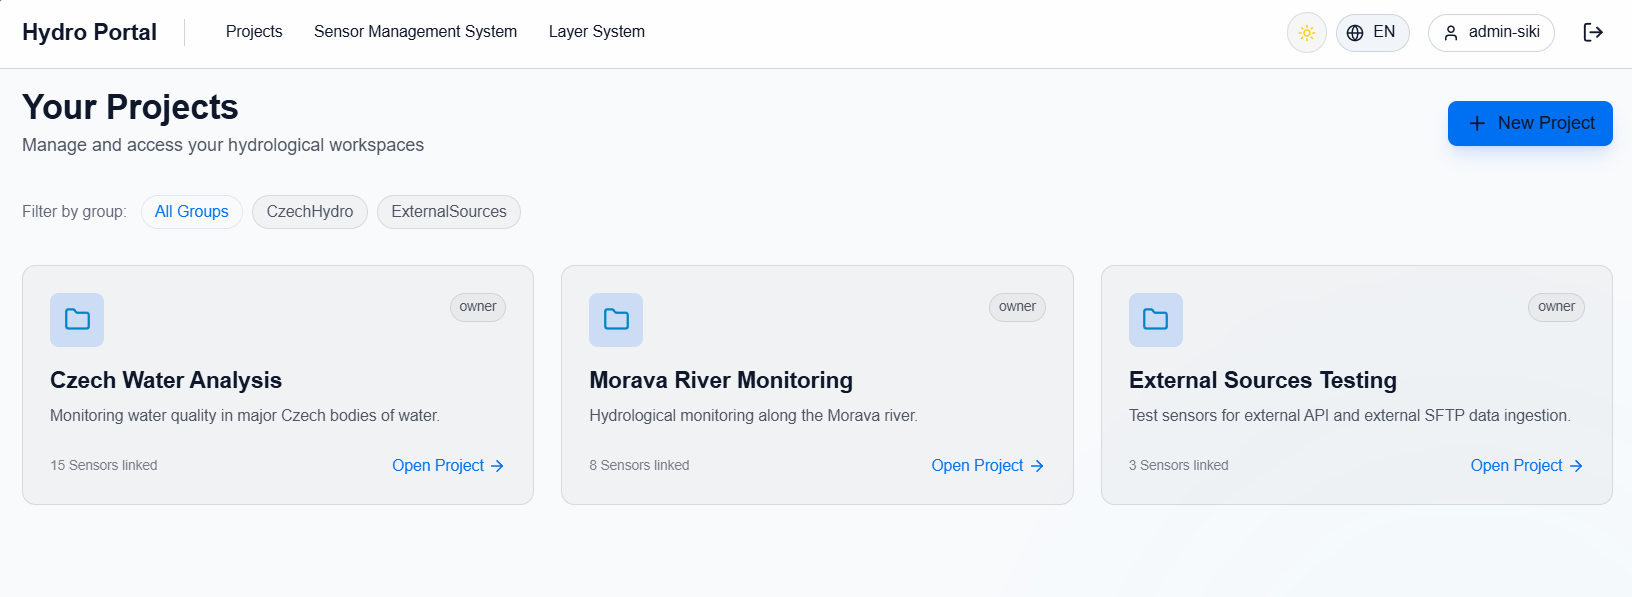
\includegraphics[width=0.95\textwidth]{figures/screenshot-dashboard.png}
  \caption{Project list page. Each card shows the project name, description,
           number of linked sensors, and the user's role. The group filter
           at the top restricts the view to a single Keycloak group.}
  \label{fig:screenshot-project-list}
\end{figure}

\subsection{Time-Series Visualization}
\label{sec:impl-frontend-charts}

Multi-series time-series data is rendered by the \texttt{TimeSeriesChart} component using the
Recharts\footnote{Recharts charting library: \url{https://recharts.org/}} library. Interactive zoom is supported via two mechanisms: a
\texttt{ReferenceArea} drawn by click-and-drag to select a time range, and a
\texttt{Brush} component for scrolling through the full dataset. Multiple series
(each with its own color, label, and unit) are merged into a unified time axis by indexing
all data points into a shared timestamp map.

Data is fetched through React~Query hooks in \texttt{hooks/queries/}, which provide
caching, background refetching, and loading-state management. Ten query-hook modules
cover the major resource types: projects, sensors, dashboards, alerts, QA/QC,
SMS, layers, simulator, and permissions. Query keys are centralized in
\texttt{hooks/queries/keys.ts} to ensure cache consistency across components.

An Axios\footnote{Axios HTTP client: \url{https://axios-http.com/}} instance in \texttt{lib/api.ts} serves as the API client, with a request interceptor that
attaches the NextAuth access token as a \texttt{Bearer} header. An in-memory token cache
with a 60-second expiry buffer avoids redundant \texttt{getSession()} calls.

Figure~\ref{fig:screenshot-sensor-detail} shows the per-project sensor detail
view for the Orl\'{\i}k Dam monitoring station. The left panel displays metadata
(status, device type, description, coordinates) and a location mini-map; the
right panel renders a time-series chart of recent observations with a datastream
selector.

\begin{figure}[ht]
  \centering
  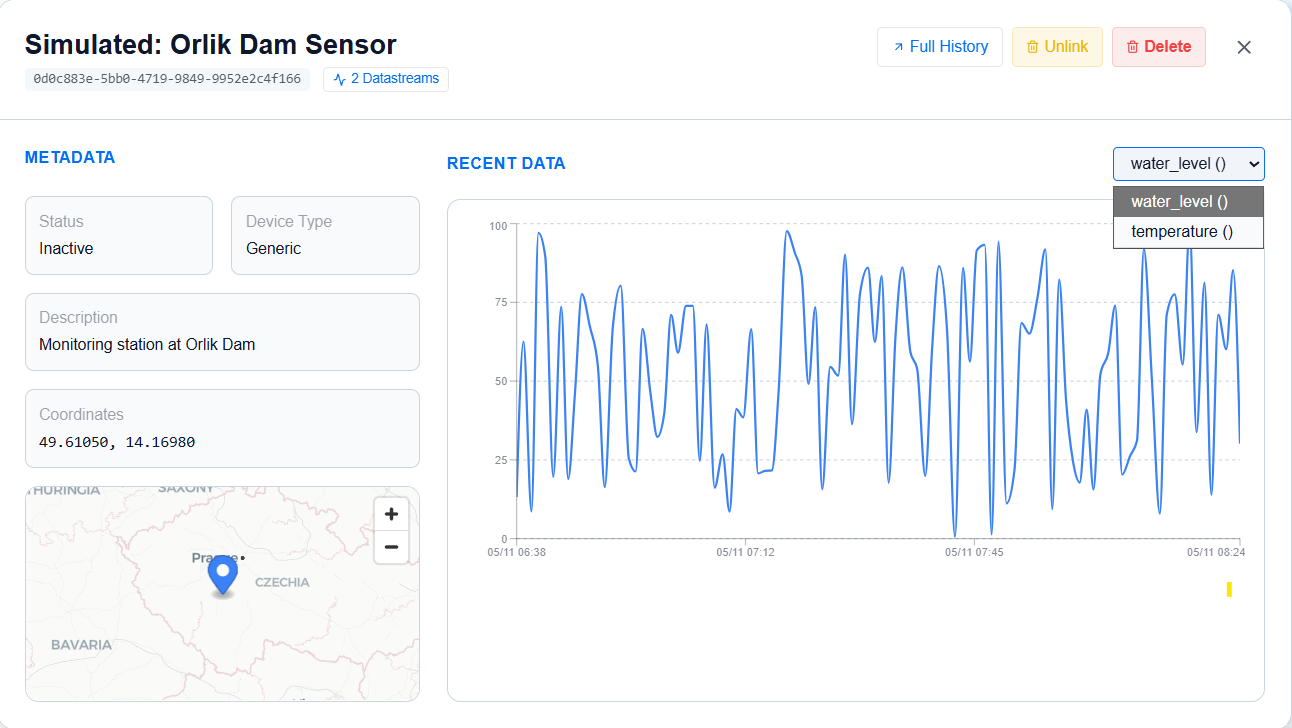
\includegraphics[width=0.95\textwidth]{figures/screenshot-timeseries.png}
  \caption{Sensor detail view within a project. The metadata panel on the left
           shows the sensor status, device type, coordinates, and a location
           mini-map. The chart on the right plots recent observations for the
           selected datastream (\texttt{water\_level}); a dropdown allows
           switching between available datastreams.}
  \label{fig:screenshot-sensor-detail}
\end{figure}

\subsection{Geospatial Layer Viewer}
\label{sec:impl-frontend-geo}

Geospatial rendering uses MapLibre~GL~JS\footnote{MapLibre GL JS mapping library: \url{https://maplibre.org/}} in three components. Sensor locations appear as clustered GeoJSON markers on a CARTO basemap
in the \texttt{ProjectMap} component
(dark-matter or positron, selected by the theme context). Marker popups show the latest
datastream values, refreshed every 30~seconds. GeoServer WMS layers assigned to the
project are overlaid as raster tiles, and a layer-switching menu allows users to
toggle their visibility.

An interactive click-or-drag marker in the \texttt{LocationPickerMap} component enables
setting sensor coordinates during Thing creation. A read-only map in \texttt{SensorMiniMap} shows the sensor's location.

Figure~\ref{fig:screenshot-map} illustrates the map view with a GeoServer WMS
layer overlay (Czech Republic boundaries) and sensor markers distributed across
the monitored region.

\begin{figure}[ht]
  \centering
  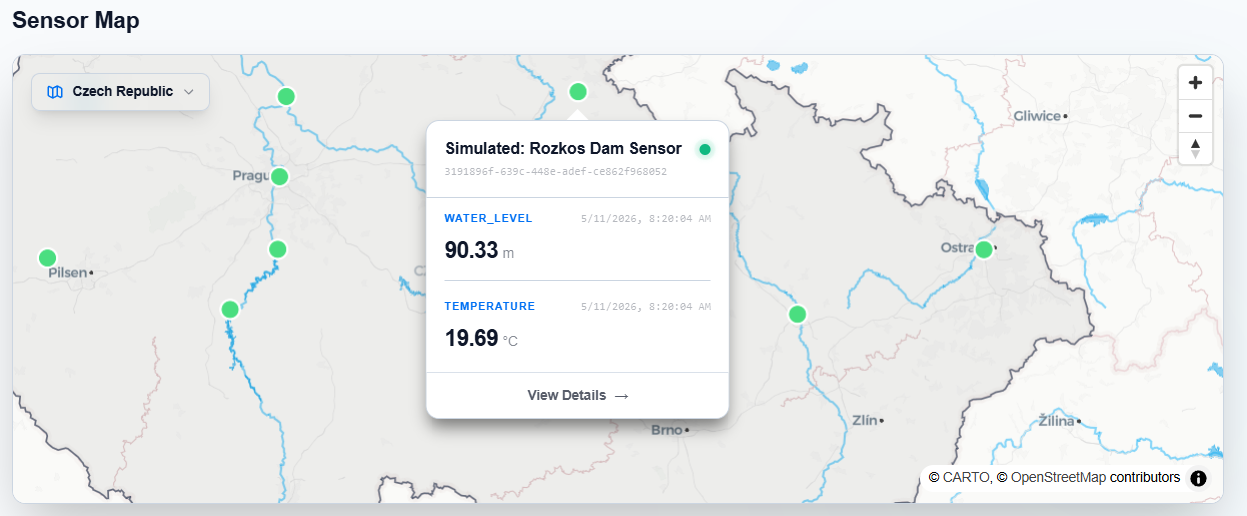
\includegraphics[width=0.95\textwidth]{figures/screenshot-map.png}
  \caption{Sensor map on a CARTO positron basemap with a GeoServer WMS layer
           overlay. The popup for the Rozko\v{s} Dam sensor shows the latest
           \texttt{water\_level} (90.33\,m) and \texttt{temperature}
           (19.69\,\textdegree{}C) readings. A layer selector in the top-left
           corner toggles WMS overlays.}
  \label{fig:screenshot-map}
\end{figure}

\subsection{Data Quality Interface}
\label{sec:impl-frontend-quality}

Accessible at two levels, per-project (\texttt{/projects/[id]/qaqc})
and globally through the SMS section (\texttt{/sms/qa-qc}), the QA/QC interface. The \texttt{SensorQAQCSection}
component renders the QC test configuration for a single sensor, allowing users to define
test types, thresholds, and parameters. A dedicated API client (\texttt{lib/qaqc-api.ts})
provides typed functions for three endpoint scopes: SMS-level, Thing-level, and
project-level QA/QC configuration.

\subsection{Batch Import}
\label{sec:impl-frontend-batch}

A drag-and-drop CSV upload workflow is provided by the \texttt{BulkImportDialog} component for
creating multiple sensors in a single operation. The \texttt{DataUploadModal} and
\texttt{DatasetUploadModal} components handle historical observation data import: users
upload CSV files which are stored in the per-Thing MinIO bucket, triggering the TSM
file-ingest pipeline. The per-sensor data view also includes a \texttt{FileUploadDialog}
for individual file uploads.

\subsection{Multilingual Support}
\label{sec:impl-frontend-i18n}

Three languages are supported by the portal: English, Czech, and Slovak. A custom solution based on a Zustand\footnote{Zustand state management library: \url{https://github.com/pmndrs/zustand}} store (\texttt{useLanguageStore}) with
\texttt{persist} middleware, which saves the selected language to \texttt{localStorage}
under the key \texttt{language-storage}. Locale files in \texttt{locales/} export typed
\texttt{Dictionary} objects (\texttt{en.ts}, \texttt{cs.ts}, \texttt{sk.ts}) that share
a common interface definition.

The \texttt{useTranslation()} hook returns a \texttt{t(path, params?)} function that
traverses the dictionary by dot-notation keys (e.g.\ \texttt{t('header.projects')}) and
supports \texttt{\{\{param\}\}} interpolation. In the application header, a \texttt{LanguageSwitcher} component allows users to switch the language at runtime.

Locale selection is purely client-side; there is no server-side locale detection or
URL-based language routing. This design was chosen to simplify the deployment and avoid
additional Next.js middleware complexity, at the cost of the initial page flash before
the persisted language is loaded from storage.

Figure~\ref{fig:screenshot-sms} shows the Sensor Management System interface, which
is accessible only to users with the \texttt{editor} role or higher.

\begin{figure}[ht]
  \centering
  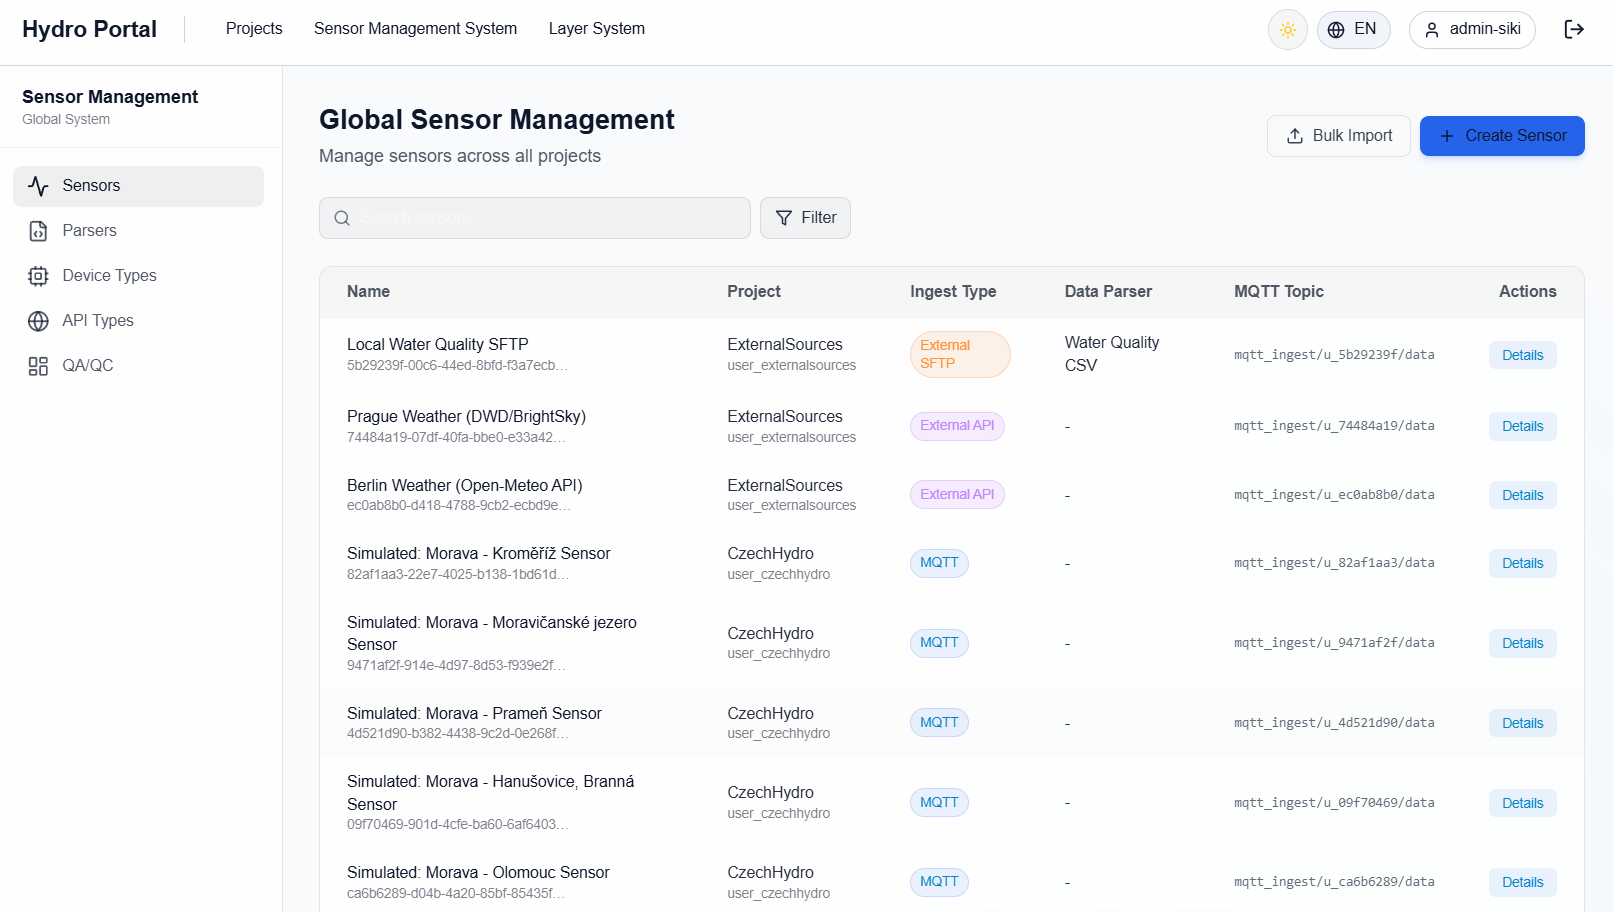
\includegraphics[width=0.95\textwidth]{figures/screenshot-sms.png}
  \caption{Global Sensor Management page in the SMS section. Each row shows
           the sensor name, owning project, ingestion type (MQTT, External~API,
           or External~SFTP), assigned data parser, and the MQTT topic. The
           sidebar provides navigation to parsers, device types, API types,
           and QA/QC configuration.}
  \label{fig:screenshot-sms}
\end{figure}

Additional portal screenshots, including SMS-level sensor detail, QA/QC
configuration, bulk sensor import, layer management, and the language switcher,
are collected in Appendix~\ref{app:screenshots}.

%% ----------------------------------------------------------------
\section{Unified Deployment Layer}
\label{sec:impl-deploy}
%% ----------------------------------------------------------------

A single entry point for deploying the full integrated platform is provided by the \texttt{hydro-deploy} repository.
It does not introduce any new runtime services; its sole responsibility is assembly and configuration.
The architectural design (Compose file merging, secret management, Makefile targets, and
Podman support) was described in Section~\ref{sec:arch-deployment}. This section covers
implementation details not addressed there.

\subsection{Compose Multi-File Merge}
\label{sec:impl-deploy-compose}

The four-file Compose chain and its merging semantics were described in
Section~\ref{sec:arch-deploy-compose}. Two implementation details warrant further
discussion.

First, the final overlay (\texttt{hydro-deploy/docker-compose.yml}) uses the YAML
\texttt{!override} tag to replace development bind-mount volumes with production-ready
empty lists, ensuring that no host paths leak into the production deployment.

Second, startup is staged by \texttt{scripts/start-docker.sh} (or
\texttt{start-podman.sh}), which brings services up in dependency order: TSM core first
(waiting for the database to become healthy), then \texttt{postgres-app}, then GeoServer
(with a 300-second timeout), then the API, and finally the worker, frontend, and optional
Cloudflare tunnel. In the Podman variant, a parallel set of \texttt{.podman.yml} files
generated by \texttt{podman\_prep.py} (Section~\ref{sec:arch-deploy-podman}) is used
instead.

\subsection{Secrets and Environment Configuration}
\label{sec:impl-deploy-env}

A single \texttt{.env} file is shared across all three repositories via symbolic links
created during setup. Cryptographic credentials are populated by the \texttt{scripts/generate-secrets.sh} script using Python's \texttt{secrets} module. Three generator functions
are used: \texttt{hex32()} for 32-byte hex tokens, \texttt{fernet\_key()} for Fernet
encryption keys (with a fallback to \texttt{base64}-encoded random bytes if the
\texttt{cryptography} library is unavailable), and \texttt{passphrase()} for 24-character
alphanumeric strings.

Credentials that must be identical across stacks are managed in synchronization groups: a
single generated database password is written to \texttt{DATABASE\_PASSWORD},
\texttt{TIMEIO\_DB\_PASSWORD}, \texttt{MQTT\_AUTH\_POSTGRES\_PASS}, and several Flyway
variables simultaneously. The script is safe to re-run: it replaces only values that still
contain the \texttt{changeme} placeholder.

Environment consistency is verified by the \texttt{scripts/check.sh} health-check script.
Five \texttt{@sync} variable pairs are validated for equality (e.g.\
\texttt{DATABASE\_PASSWORD} and \texttt{TIMEIO\_DB\_PASSWORD}). The script also checks all
containers for health status, probes HTTP endpoints for reachability, and warns about
remaining \texttt{changeme} placeholders. The derived variables (\texttt{PROXY\_URL},
\texttt{KEYCLOAK\_URL}, etc.) are computed from \texttt{PUBLIC\_HOSTNAME} and
\texttt{PUBLIC\_PORT} by the \texttt{make update-env} target using \texttt{sed}
substitutions.

\chapter{Testing and Evaluation}
\label{chap:testing}

Evaluation of the platform proceeds against the requirements from Chapter~\ref{chap:requirements}.
Section~\ref{sec:test-approach} outlines the testing strategy used. Requirements
are assessed one by one in Section~\ref{sec:test-requirements}. Performance and scalability
considerations follow in Section~\ref{sec:test-performance}, and Section~\ref{sec:test-deployment}
covers the CZU deployment and the path to eLTER adoption.

%% ----------------------------------------------------------------
\section{Testing Approach}
\label{sec:test-approach}
%% ----------------------------------------------------------------

Testing operates at three levels: automated unit and integration tests for the
data platform backend and frontend, automated tests inherited from the upstream
\texttt{tsm-orchestration} codebase, and manual end-to-end verification of the full
deployment.

\subsection{Backend Test Suite}
\label{sec:test-approach-backend}

A pytest-based test suite covering 804~test
functions across 43~test files is included with the data platform backend, organized into five directories:
\texttt{test\_api/} (endpoint-level tests), \texttt{test\_services/} (business-logic tests),
\texttt{test\_core/} (middleware, security, and exception handling), \texttt{test\_schemas/}
(Pydantic model validation), and \texttt{test\_tasks/} (Celery background tasks).

Test fixtures are defined in \texttt{conftest.py}. A \texttt{mock\_db\_session} fixture
provides a \texttt{MagicMock(spec=Session)} for SQLAlchemy interactions. The \texttt{client}
fixture creates a FastAPI \texttt{TestClient} with dependency overrides that inject the mocked
database session and an authenticated admin user, enabling endpoint tests to run without a
real database or Keycloak instance. An autouse \texttt{disable\_seeding} fixture prevents
the application from running database initialization at startup.

Custom pytest markers (\texttt{api}, \texttt{services}, \texttt{core}, \texttt{v1}) are
assigned automatically based on the test file's directory, enabling selective test execution.
By default, \texttt{pytest.ini} excludes tests marked as
\texttt{integration}, which require a live PostgreSQL instance.

Coverage is measured with \texttt{pytest-cov} against the \texttt{app/} package. The
largest test files target the most critical business logic: the TimeIO database service
(152~tests covering schema management and observation queries), the RBAC permission resolver
(76~tests covering role inheritance, batch resolution, and group-based authorization),
and the alert evaluator (69~tests covering all operators, deduplication, sensor data
evaluation, and QA/QC rule evaluation).

A Locust\footnote{Locust load testing tool: \url{https://locust.io/}}-based load testing suite is included in \texttt{tests/load/locustfile.py}. It
simulates authenticated users performing weighted API operations (project listing, sensor
queries, observation retrieval) against a running instance. The load test can be scaled
via \texttt{docker-compose.loadtest.yml}, which supports multiple Locust worker containers.

\subsection{Frontend Test Suite}
\label{sec:test-approach-frontend}

The frontend includes 96~test cases in 13~files under \texttt{frontend/\_\_tests\_\_/},
executed with Vitest\footnote{Vitest testing framework: \url{https://vitest.dev/}} and React Testing Library against a jsdom environment. The tests cover
the API interceptor (authentication header injection and error handling), React~Query hook
factories (query key generation, mutation lifecycle), and selected component rendering
(project cards). The Vitest configuration uses the \texttt{@vitejs/plugin-react} plugin
and resolves import aliases through the same path mapping used in production.

\subsection{TSM Orchestration Tests}
\label{sec:test-approach-tsm}

Upstream \texttt{tsm-orchestration} contains 131~test functions covering
parser implementations (CSV, JSON), worker scripts (file ingest, crontab setup), external
API syncers (DWD, TTN, Bosch, T-Systems, UBA), Grafana API integration, and cryptographic
utilities. These tests were inherited with the fork and continue to pass against the
modified codebase.

\subsection{Manual End-to-End Verification}
\label{sec:test-approach-e2e}

Full-stack scenarios are verified manually against a running deployment. A primary
verification path traces the complete Thing lifecycle: sensor creation through the portal,
infrastructure provisioning by TSM workers (observable through container logs and database
schema creation), data ingestion via MQTT or CSV upload, observation availability through
the FROST-Server STA endpoint, and time-series rendering in the portal charts. The
\texttt{make check} target in the deployment layer automates the infrastructure-level
portion of this verification by probing container health, HTTP endpoint reachability, and
\texttt{@sync} variable consistency.

%% ----------------------------------------------------------------
\section{Evaluation Against CZU Requirements}
\label{sec:test-requirements}
%% ----------------------------------------------------------------

Each functional and non-functional requirement from Chapter~\ref{chap:requirements} is
evaluated below. Requirements are classified as \emph{fully met}, \emph{partially met},
or \emph{not met}, with evidence from the test suite, source code, or deployed system.

\subsection{Functional Requirements}
\label{sec:test-requirements-functional}

Table~\ref{tab:req-evaluation-fr} summarizes the evaluation of functional requirements.

\begin{landscape}
{\small
\begin{longtable}{l p{0.30\linewidth} l p{0.38\linewidth}}
  \caption{Functional requirements evaluation.}
  \label{tab:req-evaluation-fr} \\
  \textbf{ID} & \textbf{Requirement} & \textbf{Status} & \textbf{Evidence} \\
  \hline
  \endfirsthead
  \textbf{ID} & \textbf{Requirement} & \textbf{Status} & \textbf{Evidence} \\
  \hline
  \endhead
  FR-1  & MQTT real-time ingestion with per-Thing parsers
        & Fully met
        & mqtt-ingest worker; parser framework with 5~device-specific parsers;
          131~upstream tests pass. \\[3pt]
  FR-2  & CSV file upload ingestion
        & Fully met
        & file-ingest worker; 13~\texttt{test\_things.py} tests cover CSV upload
          endpoint. \\[3pt]
  FR-3  & External SFTP synchronization
        & Fully met
        & sync-extsftp worker; triggered by cron via MQTT. \\[3pt]
  FR-4  & External REST API synchronization
        & Fully met
        & sync-extapi worker; DWD, TTN, Bosch, T-Systems, UBA syncers;
          30~upstream syncer tests. \\[3pt]
  FR-5  & Custom parser and syncer script upload
        & Fully met
        & Dynamic loader fetches scripts from MinIO; AST-based validation blocks
          dangerous operations. \\[3pt]
  FR-6  & Sensor CRUD with parser and coordinate config
        & Fully met
        & 25~\texttt{test\_sms.py} tests; 31~\texttt{test\_orchestrator.py}
          tests. \\[3pt]
  FR-7  & Bulk sensor import from CSV template
        & Fully met
        & \texttt{BulkImportDialog} component; 6~\texttt{test\_bulk.py} tests
          with validation and authorization checks. \\[3pt]
  FR-8  & Sensor inactivity detection and alerting
        & Fully met
        & \texttt{MonitoringService}; 51~\texttt{test\_monitoring\_service.py}
          tests. \\[3pt]
  FR-9  & Reusable MQTT device types and CSV parsers
        & Fully met
        & SMS catalog endpoints; parser/device-type CRUD tested in
          \texttt{test\_sms.py}. \\[3pt]
  FR-10 & Project CRUD with sensor grouping
        & Fully met
        & 10~\texttt{test\_project\_service.py} tests;
          6~\texttt{test\_projects.py} endpoint tests. \\[3pt]
  FR-11 & Project member roles (owner/editor/viewer)
        & Fully met
        & Two-tier RBAC; 76~\texttt{test\_rbac\_service.py} tests cover role
          inheritance and batch resolution. \\[3pt]
  FR-12 & Per-project TimeIO schema provisioning
        & Fully met
        & \texttt{TimeIOOrchestrator}; 152~\texttt{test\_timeio\_db.py} tests
          cover schema management. \\[3pt]
  FR-13 & QA/QC test pipeline configuration
        & Fully met
        & QA/QC endpoints at project and SMS scope;
          \texttt{SensorQAQCSection} frontend component. \\[3pt]
  FR-14 & Automatic QA/QC on \texttt{data\_parsed} event
        & Fully met
        & run-qaqc worker subscribes to \texttt{data\_parsed} topic. \\[3pt]
  FR-15 & On-demand QA/QC triggering via API
        & Fully met
        & QA/QC service publishes to \texttt{data\_parsed} to trigger
          re-evaluation. \\[3pt]
  FR-16 & Interactive time-series charts
        & Fully met
        & \texttt{TimeSeriesChart} component with Recharts; zoom via
          \texttt{ReferenceArea} and \texttt{Brush}. \\[3pt]
  FR-17 & Interactive map with sensor markers and WMS overlay
        & Fully met
        & \texttt{ProjectMap} with MapLibre~GL; GeoServer WMS layer overlay;
          30-second auto-refresh. \\[3pt]
  FR-19 & CSV export of Observation data
        & Fully met
        & Export endpoint in \texttt{things.py} router. \\[3pt]
  FR-20 & OIDC authentication via Keycloak
        & Fully met
        & JWKS validation in \texttt{core/security.py}; 4~\texttt{test\_auth.py}
          tests; 7~\texttt{test\_keycloak\_service.py} tests. \\[3pt]
  FR-21 & Two-tier RBAC model
        & Fully met
        & \texttt{RBACService} with six-rule priority chain;
          76~permission tests. \\[3pt]
  FR-22 & Keycloak group management
        & Partially met
        & Group management decommissioned from portal; users manage groups
          via the Keycloak admin console directly. \\[3pt]
  FR-23 & Historical CSV data upload (up to 200~MB)
        & Fully met
        & \texttt{DataUploadModal} and \texttt{DatasetUploadModal} components;
          files stored in per-Thing MinIO bucket. \\[3pt]
  FR-24 & GeoJSON geospatial import (up to 200~MB)
        & Fully met
        & Bulk import endpoint; 6~\texttt{test\_bulk.py} tests cover streaming
          and validation. \\[3pt]
  FR-25 & Multilingual UI (EN, CS, SK)
        & Fully met
        & Zustand-persisted locale store; typed dictionary files for all three
          languages. \\
\end{longtable}
}
\end{landscape}

\begin{landscape}
\subsection{Non-Functional Requirements}
\label{sec:test-requirements-nonfunctional}

Table~\ref{tab:req-evaluation-nfr} summarizes the evaluation of non-functional requirements.

{\small
\begin{longtable}{l p{0.30\linewidth} l p{0.38\linewidth}}
  \caption{Non-functional requirements evaluation.}
  \label{tab:req-evaluation-nfr} \\
  \textbf{ID} & \textbf{Requirement} & \textbf{Status} & \textbf{Evidence} \\
  \hline
  \endfirsthead
  \textbf{ID} & \textbf{Requirement} & \textbf{Status} & \textbf{Evidence} \\
  \hline
  \endhead
  NFR-1 & Containerized deployment (Docker + Podman)
        & Fully met
        & The deployment layer supports both runtimes; \texttt{podman\_prep.py}
          applies seven transformations. \\[3pt]
  NFR-2 & OGC STA compliance
        & Partially met
        & FROST-Server serves STA queries; local STA views provide entity data
          but stub views for \texttt{SENSORS}, \texttt{OBS\_PROPERTIES}, and
          \texttt{FEATURES\_OF\_INTEREST} return empty results. \\[3pt]
  NFR-3 & OIDC standards compliance
        & Fully met
        & RS256 JWKS validation with one-hour TTL cache; multi-issuer support;
          \texttt{asyncio.Lock} for concurrent refresh. \\[3pt]
  NFR-4 & Modular extensibility
        & Fully met
        & Dynamic parser loading from MinIO; runtime-uploadable syncer
          scripts. \\[3pt]
  NFR-5 & Security (script sandboxing, rate limiting, encryption)
        & Fully met
        & AST-based script validation; SlowAPI rate limiting; Fernet credential
          encryption; 10~\texttt{test\_crypto\_utils.py} tests. \\[3pt]
  NFR-6 & Maintainability (migrations, OpenAPI docs)
        & Fully met
        & Four Alembic migrations for \texttt{water\_dp} schema; Flyway for
          TSM; OpenAPI docs generated automatically by FastAPI. \\[3pt]
  NFR-7 & eLTER interoperability alignment
        & Partially met
        & STA-based data access satisfies (a); Keycloak OIDC supports federation
          with eLTER~LogIn~(b); data model is extensible for DEIMS-SDR and
          EnvThes~(c); per-site Docker~Compose deployment preserves
          autonomy~(d). No eLTER-specific metadata schemas or vocabulary
          bindings implemented yet. \\[3pt]
  NFR-8 & Unified deployment via single config
        & Fully met
        & Single \texttt{.env} with symlinks; \texttt{make up} deploys the
          full stack; \texttt{make check} validates health. \\
\end{longtable}
}
\end{landscape}

\subsection{Gap Analysis Closure}
\label{sec:test-requirements-gaps}

Table~\ref{tab:gap-closure} maps the eleven gaps identified in
Section~\ref{sec:req-gap} to their resolution status.

\begin{longtable}{l l p{0.70\textwidth}}
  \caption{Gap analysis closure.}
  \label{tab:gap-closure} \\
  \textbf{Gap} & \textbf{Status} & \textbf{Resolution} \\
  \hline
  \endfirsthead
  \textbf{Gap} & \textbf{Status} & \textbf{Resolution} \\
  \hline
  \endhead
  G-1  & Resolved & Project model with member roles and sensor assignment
         implemented in the \texttt{water\_dp} schema. \\[3pt]
  G-2  & Resolved & Next.js portal with time-series charts, maps, alerts,
         QA/QC, and sensor management. \\[3pt]
  G-3  & Resolved & GeoServer integration with REST~API layer management and
         MapLibre~GL WMS overlay. \\[3pt]
  G-4  & Resolved & Nine local STA views replace the SMS-dependent views;
         FROST-Server starts and serves valid STA responses. \\[3pt]
  G-5  & Resolved & The data platform replaces the non-functional SMS with
         sensor management endpoints and the \texttt{TimeIOOrchestrator}. \\[3pt]
  G-6  & Resolved & Alert evaluation system with sensor threshold, QA/QC, and
         inactivity rules; MQTT-triggered processing. \\[3pt]
  G-7  & Resolved & The deployment layer with Compose multi-file merge,
         \texttt{@sync} validation, and Makefile interface. \\[3pt]
  G-8  & Resolved & \texttt{podman\_prep.py} generates Podman-compatible Compose
         files; rootless-specific UID/GID and network fixes applied. \\[3pt]
  G-9  & Resolved & Three locale files (EN, CS, SK) with Zustand-persisted
         language switching. \\[3pt]
  G-10 & Resolved & \texttt{TimeIOOrchestrator} generates MQTT configuration
         messages compatible with the ingestion pipeline. \\[3pt]
  G-11 & Resolved & SMS catalog endpoints for parser and device-type CRUD;
         dynamic parser loading from MinIO. \\
\end{longtable}

All eleven gaps from the baseline analysis are resolved. Two non-functional requirements
(NFR-2 and NFR-7) remain partially met: NFR-2 due to the stub STA entity views that
return empty results for entities without a local equivalent, and NFR-7 due to the
absence of eLTER-specific metadata schemas, which are planned as future work.

%% ----------------------------------------------------------------
\section{Performance and Scalability Considerations}
\label{sec:test-performance}
%% ----------------------------------------------------------------

To validate that the platform meets its response-time target (under 2\,seconds) and
scales under concurrent load, load tests were executed using Locust~2.43 against a
local deployment of the full 22-container stack on a development machine (AMD Ryzen~7,
32\,GB RAM, NVMe SSD, Docker Desktop). Ten simulated users performed weighted API
operations (project listing, sensor queries, geospatial layer retrieval) with randomized
wait times of 1--3\,seconds between requests.

All endpoints satisfy the 2-second response time target even at the
95th~percentile (Table~\ref{tab:load-test-10u}). Lightweight CRUD operations (project
listing, project detail) maintain sub-15\,ms median latency. Endpoints that perform
HTTP fan-out to FROST-Server (\texttt{/projects/\{id\}/sensors},
\texttt{/sms/sensors}) show higher latency due to the per-Thing request pattern
discussed in Section~\ref{sec:test-perf-bottleneck}, yet remain under 310\,ms at p95.
Figure~\ref{fig:load-test-chart} visualizes the median and 95th-percentile latencies.

A follow-up test with 25~concurrent users confirmed that the application-level rate
limiter (10~authentication requests per minute per IP) correctly rejects excess login
attempts with HTTP~429 responses. Under this load, endpoints that successfully
authenticate maintain stable response times --- project listing stays at 10\,ms median,
sensor queries at 61\,ms median --- demonstrating that the API scales linearly within the
rate-limited envelope. The overall throughput reached 11.7~requests/second with
25~users.

\begin{table}[p]
  \centering
  \small
  \caption{Load test results --- 10~concurrent users, 60\,s run
           (Locust~2.43, direct API access).}
  \label{tab:load-test-10u}
  \begin{tabular}{@{} l r r r r r @{}}
    \toprule
    \textbf{Endpoint} & \textbf{Reqs} & \textbf{Avg} &
      \textbf{p50} & \textbf{p95} & \textbf{Max} \\
    & & \textbf{(ms)} & \textbf{(ms)} & \textbf{(ms)} & \textbf{(ms)} \\
    \midrule
    \texttt{POST /auth/login}          & 10  & 51  & 48  & 82   & 82   \\
    \texttt{GET /auth/me}              & 22  & 17  & 10  & 62   & 107  \\
    \texttt{GET /projects/}            & 71  & 10  & 10  & 15   & 19   \\
    \texttt{GET /projects/\{id\}}      & 34  & 8   & 6   & 11   & 45   \\
    \texttt{GET /\ldots/\{id\}/sensors} & 30 & 87 & 71  & 130  & 412  \\
    \texttt{GET /geospatial/layers}    & 16  & 104 & 79  & 280  & 280  \\
    \texttt{GET /sms/sensors}          & 27  & 103 & 51  & 310  & 1040 \\
    \midrule
    \textbf{Aggregated (valid)}        & \textbf{210} & \textbf{42} & \textbf{10}
      & \textbf{130} & \textbf{1040} \\
    \bottomrule
  \end{tabular}
\end{table}

\begin{figure}[p]
  \centering
  \begin{tikzpicture}
    \begin{axis}[
      ybar,
      bar width=10pt,
      width=0.92\textwidth,
      height=7cm,
      ylabel={Response time (ms)},
      symbolic x coords={auth/login, auth/me, projects, project detail,
                         project sensors, geo layers, SMS sensors},
      xtick=data,
      x tick label style={rotate=25, anchor=east, font=\small},
      ymin=0,
      ymax=350,
      enlarge x limits=0.08,
      legend style={at={(0.02,0.98)}, anchor=north west, font=\small},
      nodes near coords,
      every node near coord/.append style={font=\scriptsize},
    ]
    \addplot[fill=blue!50] coordinates {
      (auth/login, 48)
      (auth/me, 10)
      (projects, 10)
      (project detail, 6)
      (project sensors, 71)
      (geo layers, 79)
      (SMS sensors, 51)
    };
    \addplot[fill=orange!60] coordinates {
      (auth/login, 82)
      (auth/me, 62)
      (projects, 15)
      (project detail, 11)
      (project sensors, 130)
      (geo layers, 280)
      (SMS sensors, 310)
    };
    \legend{Median (p50), 95th percentile (p95)}
    \end{axis}
  \end{tikzpicture}
  \caption{API response time distribution under 10~concurrent users.
           Lightweight CRUD endpoints (projects, auth) respond within 15\,ms
           at p50. Data-heavy endpoints requiring FROST-Server fan-out (sensors,
           SMS) exhibit higher latency but remain well below the 2\,s threshold.}
  \label{fig:load-test-chart}
\end{figure}

\subsection{Time-Series Query Performance}
\label{sec:test-perf-timescaledb}

TimescaleDB partitions each per-thing observation table into time-based chunks. Time-range
queries, the dominant access pattern for chart rendering, benefit from chunk exclusion:
the query planner skips chunks outside the requested interval, reducing I/O to the relevant
time window. Older chunks are compressed automatically, further reducing storage requirements
and improving sequential scan throughput for historical queries.

Per-thing schema isolation provides an additional performance benefit: queries for one
sensor's data never scan another sensor's observation table, even when many sensors are
onboarded. This eliminates cross-sensor interference regardless of data volume.

\subsection{API Throughput}
\label{sec:test-perf-api}

Asynchronous request handlers with \texttt{httpx}-based FROST
client calls enable the FastAPI backend to serve multiple concurrent requests without blocking on
FROST-Server responses. The \texttt{AsyncFrostClient} maintains a connection pool
(100~maximum connections, 20~keep-alive) to reduce TCP handshake overhead for repeated
FROST queries. Under 10~concurrent users the backend sustains 4.9~requests/second
aggregate throughput; at 25~users this increases to 11.7~requests/second, confirming
near-linear scaling before the rate limiter constrains authentication-bound operations.

\clearpage
\subsection{Known Bottleneck}
\label{sec:test-perf-bottleneck}

The main performance bottleneck is the HTTP request fan-out to FROST-Server. Each
per-thing schema is served through its own FROST context path, so when the
the data platform API fetches sensor metadata for a project with many Things, it must
issue a separate HTTP request for each Thing. \texttt{AsyncThingService} mitigates
this by firing requests concurrently via \texttt{httpx} connection pooling, but the
fan-out pattern remains the throughput ceiling at scale. Adding a Redis caching layer
for frequently accessed metadata is a potential future optimization.

%% ----------------------------------------------------------------
\section{Deployment on CZU Infrastructure and eLTER Path}
\label{sec:test-deployment}
%% ----------------------------------------------------------------

On CZU infrastructure, the platform was deployed as the primary validation environment
for this thesis. This section documents the deployment, evaluates the platform's
readiness for adoption within the eLTER research infrastructure, and assesses the
long-term sustainability of the TSM-TEMP workarounds.

\subsection{CZU Deployment}
\label{sec:test-deployment-czu}

The deployment workflow described in Sections~\ref{sec:arch-deployment}
and~\ref{sec:impl-deploy} was validated on CZU infrastructure. The full stack of
22~containers was started using \texttt{make up}, with the post-deployment
\texttt{check.sh} script confirming container health, endpoint reachability across
all eight HTTP services, and credential consistency across the synchronised
\texttt{.env} variable pairs.

A platform audit conducted during this work identified and remediated 14~critical and
high-severity issues across the data platform codebase, including security header
enforcement, CORS and debug-mode controls, and credential management. An additional
27~issues were documented in the upstream TSM codebase, where remediation was not
feasible without upstream cooperation. The audit assessed all ten OWASP~Top~10
categories; accepted deferrals include the absence of a circuit-breaker pattern and
MQTT quality-of-service limited to level~1 by the upstream broker configuration.

At the time of writing, the deployment is live and publicly accessible at
\url{https://hydroportal-dev.dataraptors.eu}, where members of the CZU team are
actively accessing and evaluating the platform. This constitutes real-world validation
by the primary stakeholder group beyond automated tests and infrastructure smoke checks.

\subsection{Path to eLTER Adoption}
\label{sec:test-deployment-elter}

Several architectural properties of the platform align with eLTER requirements
described in Section~\ref{sec:bg-elter-implications}. The data access layer is built on the OGC
SensorThings API, which is a candidate standard for eLTER data exchange. Authentication
uses Keycloak with OpenID Connect, supporting the federated identity models common in
European research infrastructures. Project-based isolation provides the multi-tenancy
needed for hosting data from independent research sites. The containerized deployment
with single-file configuration enables reproducible installation across heterogeneous
institutional environments.

However, no eLTER-specific features have been implemented. The following gaps remain
between the current platform and a production-ready eLTER site-level deployment
(see Section~\ref{sec:bg-elter-ci} for the CI components referenced below):

\begin{itemize}
  \item \textbf{DEIMS-SDR site linkage.} The data model has no field for a DEIMS-SDR
    identifier, so observations cannot be linked to the eLTER site registry.
  \item \textbf{Vocabulary alignment.} Observed-property metadata is stored as
    free-text fields with no binding to EnvThes or eLTER Standard Observations.
  \item \textbf{DAR and OAR registration.} The platform cannot export metadata
    conforming to the eLTER dataset model, nor register the STA endpoint in the
    Online Asset Register.
  \item \textbf{eLTER~LogIn federation.} Keycloak would need to be configured as
    an identity broker for the eLTER~LogIn service (Perun~AAI).
  \item \textbf{Cross-site federation.} The platform operates as a single-site
    deployment; eLTER requires cross-site discovery and aggregated queries.
  \item \textbf{FAIR compliance.} Persistent identifiers (DOIs), provenance records,
    and machine-readable licensing metadata are absent.
\end{itemize}

These gaps are architectural and cannot be addressed by configuration changes
alone, but the foundational components (STA data access, OIDC authentication,
containerised deployment) are already in place for future work.

\subsection{Sustainability of the TSM-TEMP Workarounds}
\label{sec:test-deployment-tsmtemp}

The 18~\texttt{TSM-TEMP} marked locations in the codebase, concentrated in
\texttt{setup\_user\_database.py} and \texttt{sta\_views\_local/}, have shown no
operational disadvantages throughout the deployment period. The upstream SMS
service has remained non-functional throughout the duration of this thesis, and
no public roadmap for its restoration has been communicated. The assessment and
recommended migration path are discussed in
Section~\ref{sec:impl-tsm-assessment}.

\chapter{Conclusion}
\label{chap:conclusion}

This thesis addressed the problem of deploying a standards-compliant sensor data
management platform for Czech University of Life Sciences Prague within the European
eLTER research infrastructure. The existing UFZ Time.IO solution provided per-Thing
schema isolation, MQTT-driven worker pipelines, and OGC~STA data access, but lacked a
usable sensor management interface, project-level access control, and a reproducible
deployment mechanism suitable for external adopters. This work designed, implemented,
and validated a three-layer extension that fills these gaps.

\section*{Summary of Results}
\addcontentsline{toc}{section}{Summary of Results}

The implemented system consists of three independently deployable components that together
form a complete environmental monitoring platform:

\begin{enumerate}
  \item \textbf{TSM Orchestration Adaptation.}
        The upstream \texttt{tsm-orchestration} stack was adapted with local STA views
        implementing the missing FROST compatibility layer, a modular Docker~Compose
        structure enabling overlay-based configuration, and Podman rootless support for
        security-constrained infrastructure. Eighteen marked workarounds bypass the
        non-functional upstream SMS service.

  \item \textbf{The Water Data Platform.}
        A new application layer built with FastAPI (Python) and Next.js~15 (TypeScript)
        provides project-oriented sensor management, role-based access control with
        Keycloak integration, MQTT-driven alert evaluation, automated QA/QC via SaQC,
        geospatial layer integration via GeoServer, and a multilingual web portal in
        English, Czech, and Slovak.

  \item \textbf{The Unified Deployment Layer.}
        A deployment orchestrator that merges the two stacks via Docker~Compose
        multi-file merge, manages secrets, validates cross-stack configuration
        consistency, and provides a scripted operator interface via a Makefile.
        A single \texttt{make up} command starts the full 22-container stack.
\end{enumerate}

\noindent
The platform was validated through three complementary approaches:

\begin{itemize}
  \item \textbf{Automated testing.} A backend suite of 804~unit and integration tests
        covers the service layer, API endpoints, middleware, and schema validation
        (Section~\ref{sec:test-approach-backend}). All 20~functional requirements are
        fully met (Section~\ref{sec:test-requirements}).

  \item \textbf{Load testing.} Locust-based load tests with 10~and 25~concurrent users
        confirmed that all API endpoints respond within the 2-second threshold required
        by NFR-5. Lightweight CRUD operations maintain sub-15\,ms median latency;
        data-heavy endpoints involving FROST-Server fan-out remain under 310\,ms at the
        95th~percentile. The system sustains 11.7~requests/second under 25~concurrent
        users (Section~\ref{sec:test-performance}).

  \item \textbf{Deployment validation.} The full stack was deployed on CZU
        infrastructure and verified using the automated \texttt{check.sh} script, which
        confirmed container health, endpoint reachability, and cross-service
        connectivity for all 22~containers
        (Section~\ref{sec:test-deployment-czu}).
\end{itemize}

The design choice that left the deepest mark on the result was keeping
the ingestion layer and the data platform as separately deployable stacks instead of
merging them into one monolithic codebase. That separation made it possible to pull in
upstream TSM updates while letting the application layer evolve on its own. In practice,
however, the upstream Time.IO project proved unresponsive to external adopters:
the SMS service stayed broken, the frontends emitted invalid MQTT messages, and integration
documentation was absent. The data platform exists precisely because of these shortcomings.

\section*{Limitations}
\addcontentsline{toc}{section}{Limitations}

The biggest limitation is the continued reliance on \texttt{TSM-TEMP}
workarounds. Across \texttt{tsm-orchestration}, 18~marked locations bypass the non-functional
upstream SMS service with local PostgreSQL views. These views work well operationally
(Section~\ref{sec:impl-tsm-assessment}), but they carry the label of temporary fixes against a
codebase whose upstream shows no sign of addressing the root cause.

Backend test coverage, though extensive for the core service
layer (797~tests; Section~\ref{sec:test-approach-backend}), has gaps in the FROST client integration
(14\% coverage for \texttt{async\_frost\_client}) and the SMS service adapter (14\%). These
modules depend on external services that are hard to exercise without a running
FROST-Server and Keycloak instance.

Performance has not been benchmarked at scale beyond the CZU sensor fleet. The primary
bottleneck identified, HTTP request fan-out to FROST-Server's per-thing context paths
(Section~\ref{sec:test-perf-bottleneck}), would become critical at deployments with
thousands of Things. Quantitative throughput measurements under realistic multi-site load
remain future work.

Finally, the platform is not yet eLTER-ready. The architectural foundations are aligned
(OGC~STA data access, OIDC authentication, containerized deployment), but the
eLTER-specific requirements identified in Section~\ref{sec:test-deployment-elter} ---
metadata schemas, cross-site federation, vocabulary alignment, and FAIR compliance ---
represent substantial development effort beyond the scope of this thesis.

\section*{Future Work}
\addcontentsline{toc}{section}{Future Work}

What this thesis points toward is a clear next step: instead
of continuing to patch the upstream Time.IO codebase through workarounds, the more
sustainable path is to extract the \emph{architectural ideas} of Time.IO --- per-Thing schema
isolation, MQTT-driven worker pipelines, OGC~STA as the interoperability standard --- and
rebuild the problematic components from scratch, purpose-built for eLTER adoption.

The concrete future work items are:

\begin{enumerate}
  \item \textbf{TSM component rewrite.} Replace the \texttt{TSM-TEMP} workarounds
        and the non-functional SMS service with a clean STA view layer that is maintained
        as part of the platform rather than labeled as temporary. The rewrite scope is
        well-defined: 18~marked locations in one Python module and one SQL directory.

  \item \textbf{eLTER metadata integration.} Extend the project and sensor models
        with DEIMS-SDR site identifiers and EnvThes vocabulary bindings so that
        observations link to the eLTER site registry and use semantically aligned
        property descriptions. Implement metadata export conforming to the eLTER
        dataset model so that datasets can be registered in the Digital Asset
        Register and the STA endpoint listed in the Online Asset Register.

  \item \textbf{eLTER~LogIn federation.} Configure the local Keycloak instance as
        an identity broker for the eLTER~LogIn service (Perun~AAI), mapping eLTER
        roles to the platform's role model to enable single-sign-on for eLTER users.

  \item \textbf{Cross-site federation.} Implement a federation layer for aggregated
        queries across independently operated platform instances, a prerequisite for
        eLTER's distributed, multi-site architecture.

  \item \textbf{FAIR data compliance.} Add persistent identifiers (DOIs), structured
        provenance records, and machine-readable licensing metadata to support the FAIR
        data principles mandated by eLTER.

  \item \textbf{Performance optimization.} Introduce a caching layer (Redis) for
        frequently accessed FROST metadata, evaluate FROST-Server alternatives or
        clustering, and conduct load testing at scale beyond the CZU sensor fleet.

  \item \textbf{Test coverage completion.} Extend the automated test suite to cover the
        FROST client integration and SMS service adapter, potentially using
        containerized test fixtures (Testcontainers) for FROST-Server and Keycloak.
\end{enumerate}

\medskip\noindent
The OGC SensorThings API proved to be a well-chosen interoperability standard for this class
of environmental monitoring platform. Its entity model maps naturally onto the sensor data
management domain, and the availability of the FROST-Server implementation reduced the
initial integration effort. The primary friction was not with the standard itself but with
the state of the upstream implementation layer that was intended to bridge it to operational
sensor networks. The experience of this thesis suggests that the concept behind Time.IO ---
a modular, MQTT-driven, STA-compliant sensor data platform --- is sound, but a purpose-built
implementation targeting eLTER's specific requirements would be more effective than continued
adaptation of an upstream codebase that does not prioritise external adopters.


\printbibliography[heading=bibintoc]

\end{document}
